% aa.dem % AA vers. 9.1, LaTeX class for Astronomy & Astrophysics % demonstration file % (c) EDP Sciences 
%-----------------------------------------------------------------------
%
%\documentclass[referee]{aa} % for a referee version
%\documentclass[onecolumn]{aa} % for a paper on 1 column
%\documentclass[longauth]{aa} % for the long lists of affiliations
%\documentclass[letter]{aa} % for the letters
%\documentclass[bibyear]{aa} % if the references are not structured % according to the author-year natbib style

%
\documentclass{aa}  
% SRK website: 42FC36A2
%
\usepackage{graphicx,svg,bm,amsmath,dsfont,siunitx,wasysym,tikz,color,scalerel,multirow,tabularx,hyperref,placeins}
%%%%%%%%%%%%%%%%%%%%%%%%%%%%%%%%%%%%%%%%
%\usepackage{comment}
%\usetikzlibrary{arrows,positioning,decorations.pathmorphing,backgrounds,calc,shadows}
%\tikzset{
%    ashadow/.style={opacity=.25, shadow xshift=0.1, shadow yshift=-0.1, color=red!50!black},
%    block/.style={rectangle, draw=black, left color=black!20, right color=green!60!, very thick, inner sep=1, outer sep=0, minimum width=25mm, text width=25mm, minimum height=20mm, text centered, drop shadow={ashadow}, rounded corners=2mm},
%    largeblock/.style={rectangle, draw=black, left color=black!20, right color=green!60!, very thick, inner sep=1, outer sep=0, minimum width=40mm, text width=40mm, minimum height=20mm, text centered, drop shadow={ashadow}, rounded corners=2mm},
%    largeblock2/.style={rectangle, draw=black, left color=black!20, right color=green!60!, very thick, inner sep=1, outer sep=0, minimum width=50mm, text width=50mm, minimum height=20mm, text centered, drop shadow={ashadow}, rounded corners=2mm},
%    textarea/.style={rectangle, draw=black, top color=cyan!30, bottom color=cyan, very thick, inner sep=1, outer sep=0, minimum width=25mm, text width=25mm, minimum height=15mm, text centered, drop shadow={ashadow}, rounded corners=1mm},
%    textarea2/.style={rectangle, draw=black, top color=cyan!30, bottom color=blue!50, very thick, inner sep=1, outer sep=0, minimum width=25mm, text width=25mm, minimum height=15mm, text centered, drop shadow={ashadow}, rounded corners=1mm},
%    textarea3/.style={rectangle, draw=black, top color=green!30, bottom color=cyan, very thick, inner sep=1, outer sep=0, minimum width=25mm, text width=25mm, minimum height=15mm, text centered, drop shadow={ashadow}, rounded corners=1mm},
%    largetextarea/.style={rectangle, draw=black, top color=blue!30, bottom color=magenta, very thick, inner sep=1, outer sep=0, minimum width=50mm, text width=50mm, minimum height=15mm, text centered, drop shadow={ashadow}, rounded corners=1mm},
%    largetextarea2/.style={rectangle, draw=black, top color=blue!30, bottom color=green!50, very thick, inner sep=1, outer sep=0, minimum width=50mm, text width=50mm, minimum height=15mm, text centered, drop shadow={ashadow}, rounded corners=1mm},
%    picframe/.style={rectangle, draw=black, thick, inner sep=0, outer sep=0},
%    dummy/.style={inner sep=0, outer sep=0, minimum width=0, minimum height=0},
%    myarrow/.style={->, >=latex', shorten >=1pt, very thick},
%    arrow/.style={=>, >=open triangle 90, very thick}
%}

%%%%%%%%%%%%%%%%%%%%%%%%%%%%%%%%%%%%%%%%
%\usepackage[options]{hyperref}
% To add links in your PDF file, use the package "hyperref"
\definecolor{midblue}{rgb}{0.0,0.4,0.7}
\definecolor{midgreen}{rgb}{0.0,0.8,0.3}
\definecolor{mypurple}{rgb}{0.8,0.2,0.8}
\definecolor{midorange}{rgb}{0.8,0.4,0.0}
\newcommand{\edits}[1]{\textcolor{midblue}{#1}}
\newcommand{\fg}[1]{\textcolor{midblue}{#1}}
\newcommand{\fag}[1]{\textcolor{midpurple}{[FAG: #1]}} % with options according to your LaTeX or PDFLaTeX drivers.
\newcommand{\mjk}[1]{\textcolor{midgreen}{[MJK: #1]}} % with options according to your LaTeX or PDFLaTeX drivers.
\newcommand{\skk}[1]{\textcolor{midorange}{[SKK: #1]}} % with options according to your LaTeX or PDFLaTeX drivers.
%
\newcommand{\arrc}[1]{\begin{matrix}[c] #1 \end{matrix}}
\newcommand{\eqnl}[2]{\begin{eqnarray}\label{#1}#2\end{eqnarray}}
\newcommand{\floor}[1]{\left\lfloor #1 \right\rfloor}
\newcommand{\intef}[4]{\int \limits_{#1 = #2}^{#3} \! #4 \, \mathrm{d} #1}
\newcommand{\intes}[4]{\operatorname{\Bigg|} \limits_{#1 = #2}^{#3} \!\!\!\!\! #4}
\newcommand{\ave}[1]{\langle #1 \rangle}
\renewcommand{\min}[1]{\operatorname{min} \left\{ #1 \right\}} 
\renewcommand{\max}[1]{\operatorname{max} \left\{ #1 \right\}} 
\newcommand{\dd}[0]{\mathrm{d}}
\definecolor{midpurple}{rgb}{0.7,0.1,0.7}
\newcommand{\s}[2]{{#1}_{\mathrm{#2}}}
\newcommand{\RA}{{\mathsf{RA}}}
\newcommand{\Dec}{{\mathsf{Dec}}}
\newcommand{\dR}{{\mathsf{\delta RA}}}
\newcommand{\dD}{{\mathsf{\delta Dec}}}


\begin{document} 

%MJK I would reform to "Forty years of Metsähovi radio observatory data of the Sun in the 37 GHz band"
%SKK There already is a paper of almost identical name
%MJK oh, but is this not then paper number II in that series? I mean, the title now binds us to presenting the radio butterfly diagram only. But I guess this is more or less the intent anyways.
  \title{Radio butterfly diagram from 40 years of Metsähovi solar observations
         on 37 GHz}
 
  \subtitle{I. Determining bias for Earth's atmosphere, solar limb brightening,
            and antenna beam convolution}
 
  \author{
    Sami Kivistö \inst{1,2}
    \and
    Merja Tornikoski \inst{1}\fnmsep
      \thanks{Contributions to antenna beam definition}
    \and
    Joni Tammi\inst{1}
    \and
    Juha Kallunki\inst{1}
    \and\\
    Maarit Käpylä\inst{2,3,4}
    \and
    Frederick Gent\inst{2,5}
  }

  \institute{
    Mets\"ahovi Radio Observatory (MRO), Aalto University,
      Mets\"aovintie 114, 02540 Kylm\"al\"a, Finland
    \and
    Department of Computer Science, 
    Aalto University, PO Box 15400, 00076, Finland
         \email{sami.k.kivisto@aalto.fi}
    \and
    Max Planck Institute for Solar System Research,
      Justus-von-Liebig-Weg 3, 37077 G\"ottingen, Germany
    \and 
    Nordic Institute for Theoretical Physics,
      Roslagstullsbacken 23, 106 91 Stockholm, Sweden 
    \and 
    School of Mathematics, Statistics and Physics,
      Newcastle University, NE1 7RU, UK 
  }
  \date{Received \today; accepted \today}

% \abstract{}{}{}{}{} 
% 5 {} token are mandatory
 
  \abstract
  % context heading (optional)
  % {} leave it empty if necessary  
  {
    Mets\"ahovi Radio Observatory has collected solar intensity maps for
    over $40$ years.
    Most data coverage is on $\SI{37}{GHz}$ frequency band.
    This data allows for analysis and identification of features over nearly
    four sunspot cycles, constituting roughly two solar magnetic cycles.
  }
  % aims heading (mandatory)
  %MJK Method paper: the aim should be to develop a method to extract some information from the data. Butterfly diagram is, as I understand, the only end product that we want to mention. That should perhaps be in the Results section of the abstract, right?
  {
    Analyze Metsähovi solar maps for years 1978 to present.
    Investigate for any features that would correlate with magnetic and
    sunspot activity.
  }
  % methods heading (mandatory)
  %MJK Method oriented paper: Detect HOW, Collapse HOW, Quantify HOW, Compare HOW
  %FAG The methods abstract needs to be compressed and most of this detail 
  %moved to the main text. Fred TODO
  %MJK Yes. It is good to bear in mind that the arXiv abstract field allows for 1920 chars... As we will submit there anyways, then it will be an additional pain, so better to conform to the char limits already now.
  {
   %FAG moved section to disk fitting
    %Determine the solar disk position and size from each map as well as
    %normalise the measured background intensity for zero and the Quiet Sun
    %Level (QSL) for unity.
    %This can be done using a binary combination of two disk methods (1 and 
    %2) and three normalisation methods (a, b, and c).
    %The methods are: (1) intentionally weighted center of mass of the radio
    %sample coordinates, (2) fitting a circle for those sample coordinates
    %which we, by geometry, expect to belong to the solar limb, (a) sort the
    %intensity samples and detect the point of zero curvature from the index vs.     intensity dependency, the S-curve, (b) iteratively calculate the
    %statistical mean and standard deviation of the intensity of 
    %those points which are located within the solar disk and not too close
    %to the limb, (c) detect two significant peaks from the intensity histogram,
    %the lower intensity peak being the background and the higher the QSL.

    %The method (2) can be augmented using two additional sets of information.
    %When we observe exactly at the limb, we would expect $0.5$ QSL intensity
    %due the the beam mixing disk and background signal.
    %If one particular sample has intensity $0.4$ QSL, we would expect the
    %sample to be slightly more away from the center.
    %Collecting a large set of observations on different conditions, we can
    %estimate how quickly the intensity drops as the beam passes the limb 
    %from disk to background.
    %Utilizing this limb profile, we can fine tune the position of each limb
    %sample in the target set of (2) and proceed iteratively to obtain more
    %accurate circle fitting.

    Any exceptional bright or dim features near the limb will affect the
    apparent shape of the solar disk in the map. 
    They will affect the outcome of the disk center position when we run the
    circle fitting algorithm.
    Bright features favour center fitting towards the feature,
    while dim features repel the center.
    We should thus exclude a specimen from the target set of the circle fitting
    by proximity of any pre-determined bright or dim radio feature, since these
    features affect the apparent shape of the disk.
   
    Each radio specimen is given heliographic coordinates as well as time of
    observation.
    We collect a two-dimensional histogram where each rectangular slot has a
    time range as well as a range of heliographic latitude.
    Integrating all the radio data, we aim to obtain a diagram analoguous to
    the famous butterfly diagram of sunspot activity.
    Assuming the diagram will have similar wing patterns as the sunspot
    butterfly, we will apply a feature detection for wing elements.
    We apply the same algorithm for the sunspot butterfly and compare the shape
    and duration of each wing.
  }
  % results heading (mandatory)
  {
    Radio butterfly diagram on $\SI{37}{GHz}$ frequency band.
    Identified solar cycles 21 to 24.
    Wing parameters from both the radio butterfly and the sunspot butterfly.
  }
  % conclusions heading (optional), leave it empty if necessary 
  %MJK This part sounds very good
  {
    We have developed a method for automatic feature detection from butterfly
    diagrams.
    This allows systematic comparisons between individual wings as well as
    different observational and simulated datasets showing butterfly a pattern.
  }

  \keywords{Solar physics, radioastronomy, butterfly diagram, solar cycle}

  \maketitle
%-------------------------------------------------------------------
    


\section{Introduction}

  %MJK References required. FAG: added, sufficient?
  The solar magnetic field is known to switch polarity in a full cycle of 
  approximately % ca. FAG abbr. -->  full word convention
  22 years, which consists of two sunspot cycles \citep{HEN19,Babcock61}.
  At %In FAG In --> At
  the beginning of each sunspot cycle, the solar magnetic field is an axial
  dipole.
  %FAG reworded
  %Due to differential rotation, this field, being dominantly axisymmetric and running mainly in meridional planes, hence being dominantly 
  %poloidal, is transformed into an azimuthal field with the azimuthal direction being opposite between opposite hemispheres.
  %Solar differential rotation transforms the predominantly axisymmetric
  %Poloidal magnetic field into an azimuthal field with a 
  %MJK typo tendancy; but is it only a tendency? 
  %FAG: I interpreted tendency as approximate; reworded to avoid ambiguity
  %tendency
  %for opposite
  %polarity between hemispheres.
  Solar differential rotation transforms the predominantly axisymmetric
  poloidal magnetic field into an azimuthal field with opposite
  polarity between hemispheres.
  %MJK This is the controversial part of the solar dynamo process, and we need to think how to phrase things here.
  In the presence of convection and the Coriolis force due to solar rotation,
  %FAG consistent tense
  %this azimuthal field will be further distorted by the $\alpha$-effect.
  this azimuthal field is further distorted by the 
  %MJK Needs clarification in words before bluntly introducing alpha effect. Also references are needed here.
  %FAG: added in response to MJK
  action of turbulent vortical flows stretching, twisting and looping the field,
  known as the 
  $\alpha$-effect \citep{SKR66,KR80}.
  %After ca. $11$ years, this has resulted in dipolar field of opposite polarity, 
  %FAG ca. --> appr, and tense
  %After approximately 11 years this evolves into a dipolar field with
  %MJK whereto 'this' refer is unclear.
  %FAG: clarified
  After approximately 11 years the large scale magnetic field
  evolves into a dipolar field with
  polarity reversed from its original sign
  and the next sunspot cycle begins.
  %FAG remove paragraph break and reword
  The full 22 year cycle comprises two such sunspot cycles.
  
  %The full magnetic cycle is ca. $22$ years and consists of two sunspot cycles.

  %FAG insert paragraph break
  %Each sunspot cycle begins with 
  %an axial dipole, after which various activity on the visible surface of the Sun will first increase, 
  %then reach maximum and again decrease to a minimum, while it migrates from high latitudes towards the equator. This is 
  %FAG reword the Sun --> Sun NASA capitalization convention
  %Each sunspot cycle emerges from the quiet Sun of an axial dipole as
  %MJK 'emerges from the quiet Sun of an axial dipole' sounds a bit odd.FAG: rephrased 
  Starting from a quiet Sun containing a relatively weak axial dipole,
  each sunspot cycle emerges as
  activity on the visible surface of the Sun, typically near mid-latitudes
  %FAG Moved from below
  ($\pm20^{\circ}$ to $\pm 30^{\circ}$).
  While the frequency and coverage of the sunspots increases towards a maximum,
  the location of the activity drifts equatorward. 
  This migration continues after the maximum with decreasing activity
  closer to the equator, bringing the sunspot cycle to an end.
  This was first recorded in the Maunder butterfly diagram by Edward Maunder
  in 1904.
  %FAG: moved from below
  Since sunspots are a feature of Sun's magnetic field, and as the solar
  magnetic field is mostly axisymmetric, 
  %MJK References needed here FAG: OK?
  the longitudinal location of the
  activity can reasonably be neglected \citep{PBKT06}.
  Considering this two-dimensional time-latitude histogram of sunspot activity
  or magnetic field intensity, similar butterfly 
  diagrams are also recovered from solar magnetograms
  %MJK Streamline the referencing here.
  %\citep{GHHZ83,VLMCS12}
  %and \citep[][and references therein]{LUSDADM17}.
  \citep{GHHZ83,VLMCS12,LUSDADM17}.
  It is also reported for radio brightenings of the 17 and $\SI{34}{GHz}$ band
  \citep{Shibasaki13,SCGVPS14} and of $\SI{37}{GHz}$ \citep{metsahovi40}.
  \fag{add additional references in radio and visible data into above paragraph}
  Other wavelengths  \citep{Loukitcheva19} 
 
  %FAG comment below duplication
  %%MJK I think the toroidal field is evolving all the time; maybe better is to say during the dominance of the toroidal field?
  %
  %During the time of evolving azimuthal field, we observe various types of activity, such as sunspots, magnetic regions as well as radio brightenings. These features appear first in the middle latitudes ($\pm 
  %20^{\circ}$ to $\pm 30^{\circ}$) on both hemispheres. 
  %
  %%MJK Now the impression is that the distribution is bimodal; only at high and then only at low. Maybe to add 'progressively closer'
  %
  %Later in the cycle, they appear closer to the equator. 
  %%MJK I would say something on the lines: '
  %
  %%FAG moving this into the previous paragraph above
  %As the solar magnetic field is mainly axisymmetric, a longitudinal average is suitable. Taking such an average, resulting in a two-dimensional time-latitude histogram, reveals the preferred locations of magnetic activity on patterns that resemble butterfly wings...
  %The 
  %density of a preferred activity will be integrated into a two-dimensional histogram, which show the average density as a 
  %function of time and heliographic latitude. This is known as a butterfly diagram, and was first constructed for 
  %%MJK Kallunki papers are most likely not sufficient reference for the magnetic butterfly diagrams, only for radio brightenings. 
  %sunspots and later for magnetic regions and radio brightenings \cite{metsahovi40}.
 
  %FAG adding addition context
  From sunspots and magnetograms of the photosphere we have relatively rich
  %MJK hyphen ?
  %well resolved 
  well-resolved
  data about the 
  %MJK should perhaps be written out, when used for the first time, same for 3D.
  %FAG:OK done
  two-dimensional (2D) 
  evolution of the solar surface magnetic 
  field, but observation of the three-dimensional (3D)
  structure of the field is limited by the 
  weakness of magnetic measurements from the solar atmosphere relative to the
  surface.
  %FAG reworded and expanded 
  Mets\"ahovi radio observatory (MRO)\footnote{
  \href{https://www.aalto.fi/en/metsahovi-radio-observatory}{
        https://www.aalto.fi/en/metsahovi-radio-observatory}}
  is observing emissions, primarily in
  $\SI{37}{GHz}$ frequency band, dating back over forty years.
  This is in the frequency range suitable for detecting non-thermal emissions
  from high energy electrons associated with active-region magnetic fields, so %SKK 'so is' -> 'which makes it' maybe?
  is a good proxy for the intensity of the magnetic field.
  These are also well suited to observing the thermal emissions from the quiet
  Sun.
  Comparing and contrasting the maps from these emissions with other
  observations can help to reveal more about the structure of the magnetic
  field in plasma of varying temperature and by inference height.
  Furthermore, the data incorporates almost four magnetic cycles, yielding
  a valuable resource to investigate long-term variation within and between 
  cycles, alongside and in contrast to other sources.
  %Metsähovi radio observatory (MRO) has collected solar maps since 1978. Most of these maps are recorded on 
  %%MJK Fred is better with the language, but I make the following notions:
  %%MJK 'in 37 GHz frequency band', 'a valuable', 'long-term'
  %$\SI{37}{GHz}$, which is valuable resource for analyzing long term solar evolution.
  %%MJK What kind of solar activity does 37GHz trace? This is an important point to clarify.
  %FAG added new para break

  \fag{add paragraph reviewing previous Mets\"ahovi publications and references}
  %MJK One should explain in more detail what Kallunki has already published from this data.

  %FAG I have summarised the rest of the introduction to keep it concise and
  % have copied the rest to the methods section, where it is better suited.
  Across the lifetime of the MRO the equipment has experienced several upgrades
  and evolution of the data format.
  This article shall describe the pipeline of data processing to transform the
  raw data into a time series of solar radio maps, normalised, corrected for
  instrumental bias, atmospheric noise and effects, time of day and seasonal
  effects and solar limb dimming effects.
  We present two methods for correctly detecting the position of the solar disk
  in each map and three methods for normaliseing the signal levels, such that
  the background \emph{black sky} has value zero and the 
  %FAG: expanded definitiion in response to MJK later query
  %Quiet Sun Level (QSL) value unity.
  Quiet Sun Level (hereafter QSL),
  the solar intensity in the absence of surface magnetic activity, has
  value unity.
  The maps are then projected from RA and Dec onto their rotating heliographic
  surface coordinates.
  We also introduce tools we have prepared for automatic tracking of active 
  regions, which are suitable for any magnetograms or similar maps, and which
  we shall apply in detail in future publication.
  This is described in Section\,\ref{sect:methods}.

  %MJK 'From this' does not sound understandable. 
  %From this we present a time-latitude histogram of the radio intensity,
  %FAG: reduced
  We present a time-latitude histogram of the radio intensity,
  including previously inaccessible machine-drawn maps from 1978 -- 1987 and
  up to 2020.
  This yields the most complete time series thus far available from MRO, 
  spanning almost completely the last four sunspot cycles.
  We compare our butterfly diagram with one constructed from the sunspot 
  counts during the same epoch.
  These are presented in Section\,\ref{sect:results} together with some 
  examples of our active region tracking.
  Finally, we discuss in Section\,\ref{sect:discussion} 
  %%MJK some 
  %how the radio 
  %observations differ from other solar observations, 
  %%MJK Consistency with Shibasaki could be left to be said later.
  %consistent with the 
  %results of \citet{Shibasaki13}. 
  %FAG: response to MJK 
  how MRO observations differ from some other solar observations, 
  %MJK Consistency with Shibasaki could be left to be said later.
  and also compare with the results of \citet{Shibasaki13}. 

  %FAG the residual text has been copied to Methods 
  %During the 40 years, the equipment 
  %has experienced several upgrades and there has also been changes in the data format.
  %he data requires careful 
  %normalisation procedures, after which the butterfly diagram can be constructed from the solar maps. The solar maps from 
  %1978 to 1987 were originally recorded on magnetic tapes, out of which the data was rendered on contour maps using a 
  %mechanical plotter. Since then, the magnetic tapes have been lost, and the maps were only available as 
  %%MJK it would not hurt to stress that they were printer on paper only -> plots -> printouts.
  %these plots.
  %%MJK or rather pattern recognition?
  %Using various image recognition techniques featured in \cite{masterthesis}, these contour maps were converted back into 
  %numerical form. For these prepared contour maps, 
  %%MJK Define better what you mean by 'solar disk being available'. It might not be clear to a common reader.
  %the solar disk was already available, while for the later maps from 
  %1989 to present the disk 
  %has to be detected using automatic image recognition. 
  %%MJK To make it more clear:
  %%MJK The purpose of this paper is to present two methods () for detecting the disk and ....
  %We present two methods (1: S-curve and 
  %center of mass, 2: convex hull) for detecting the disk and three methods (a: S-curve and constant fraction, b: 
  %statistics and outlier neglection, c: interpolating between histogram peaks) for normaliseing the signal levels so that 
  %zero is the black sky at the background and unity is the Quiet Sun Level (QSL).
  %%MJK Then there should be a sentence stating that "As our final data product we present here a butterfly diagram of radio brightenings extending over the full time span of the recorded Mets\"ahovi solar data set".
  %
  %%MJK This would be better in the methods section, to outline the general workflow from the raw data to the final product.
  %When the disk fitting is done, every radio sample can be projected into rotating heliographic surface. We use the 
  %Carrington coordinates for this. As every sample now has time, heliographic latitude, and intensity relative to QSL, we 
  %can average them on a two-dimensional grid in order to obtain a butterfly diagram. The sunspot data is already in a 
  %format that has latitude and time bins, so simple interpolation is needed to convert it into the same domain as our 
  %butterfly. For radio data, the measurable quantity is the intensity, while for the sunspot data it is the fraction of 
  %area covered by sunspot, between two arcs of constant latitude.
  %
  %Having obtained the butterfly 
  %%MJK diagram?
  %diagrams, we 
  %%MJK We should imply that more analysis is to come later.
  %%MJK "We also perform a preliminary analysis of the obtained butterfly diagram, by performing feature detection algorithm ... that is discussed in section BLAA. Our preliminary findings are presented in Section BLAA2."
  %perform feature detection in order to get quantified information on the wing 
  %shapes. 
  %%MJK Again, introduction might not be the best place to describe the workflow, but the methods section.
  %This is done iteratively, starting with the each hemisphere and predefined solar cycle start and end times 
  %(later: wing). For each wing, we give the high intensity cells a considerable weight and fit a polynomial of a desired 
  %degree to the time-latitude domain. This gives the wing shape and root. Statistical variance with respect to the root 
  %gives us the wing thickness, which can be assumed a constant or a polynomial function of desired degree. We fit the 
  %third polynomial in the time,intensity domain, where the intensity is averaged over the wing latitudes for each time 
  %cell. The relevant roots or local minima of this intensity polynomial give the begin and end times for each wing. Having 
  %now quantified the shape and dimensions of each wing, we can neglect any outlier cells from the grid and perform several 
  %iteration steps to refine the shape. In the last stage, all the wings will coexist in the same grid, which now contains 
  %all the 40 years of data from both hemispheres. We will set the weights to zero for those cells which would have 
  %overlapping wings, in order to encourage the algorithm to produce non-overlapping wings. We tried several sets of 
  %parameters, while the most promising fits were produced with first order wing shape and thickness and fourth order 
  %intensity profile.
  %
  %%MJK So, to summarize my comments to the intro: expand significantly on Kallunki earlier paper(s), and pinpoint in detail what was there, and what is new in here, and why this work was necessary. Expand on the relevance of the dataset: what does 37GHz data describe, why is it relevant, what else has been done before in the frequency band? Move the parts describing the workflow to Section 2.
  %
\section{Methods}\label{sect:methods}

\fag{Explain here which steps are not used for historical maps and which analysis in the paper below applies to the new maps and the old maps - tracking not feasible
Summarise the pipeline and the reasons for each step in a paragraph here before then detailing the steps.
identify coordinates -- information about the chromosphere with lim brightening
model, and estimate radius of the radio data, etc.
}

\subsection{The solar maps}\label{sect:source}


  During a typical measurement, the antenna beam makes a sweep across the
  visible solar disk (Fig.~\ref{typicalmap}). There are three major sets of conventions during the history the record.
  \begin{enumerate}[A]
    \item
    The solar maps from 1978 to 1987 were originally recorded on magnetic
    tapes, from which the data was rendered onto paper contour maps using a
    mechanical plotter.
    Subsequently the magnetic tapes were lost, so that only the printed maps
    were available. Applying pattern recognition techniques presented in \cite{masterthesis}, scans of the maps were converted into
    %MJK This might not be understandable stand alone. One could add smthg like "the digital format currently used for reconrding new maps".
    %FAG: reworded as suggested
    a digital format, which is compatible new maps.
    The solar disk position as well as the rotational axis was already marked on these paper maps using a compass and a ruler.
    \item
    Until the end of May 2015 the maps were scanned in the equatorial direction,
    so that declination is shifted between adjacent sweeps, as displayed in
    Fig.~\ref{typicalmap}{\bf(a)}.
    The maps assume linear antenna tracks with constant speed and sample rate.
    \item
    After June 2015 the sweeps have been horizontal, with shifting altitude
    between sweeps, as shown in Fig.~\ref{typicalmap}{\bf(b)}.
    These modern maps respect the true path of the antenna, typically recorded
    with $25$ samples per second for two minutes.
    %MJK The final map in solar coordinates is presented in Fig.1(c)...
    %The final map in solar coordinates is presented in Fig\ref{typicalmap}{\bf(c)}.
    %SKK: Currently we have no carrington maps planned to be shown on the paper
  \end{enumerate}

%--------------------------------------------------------------------
  \begin{figure}
  \centering
  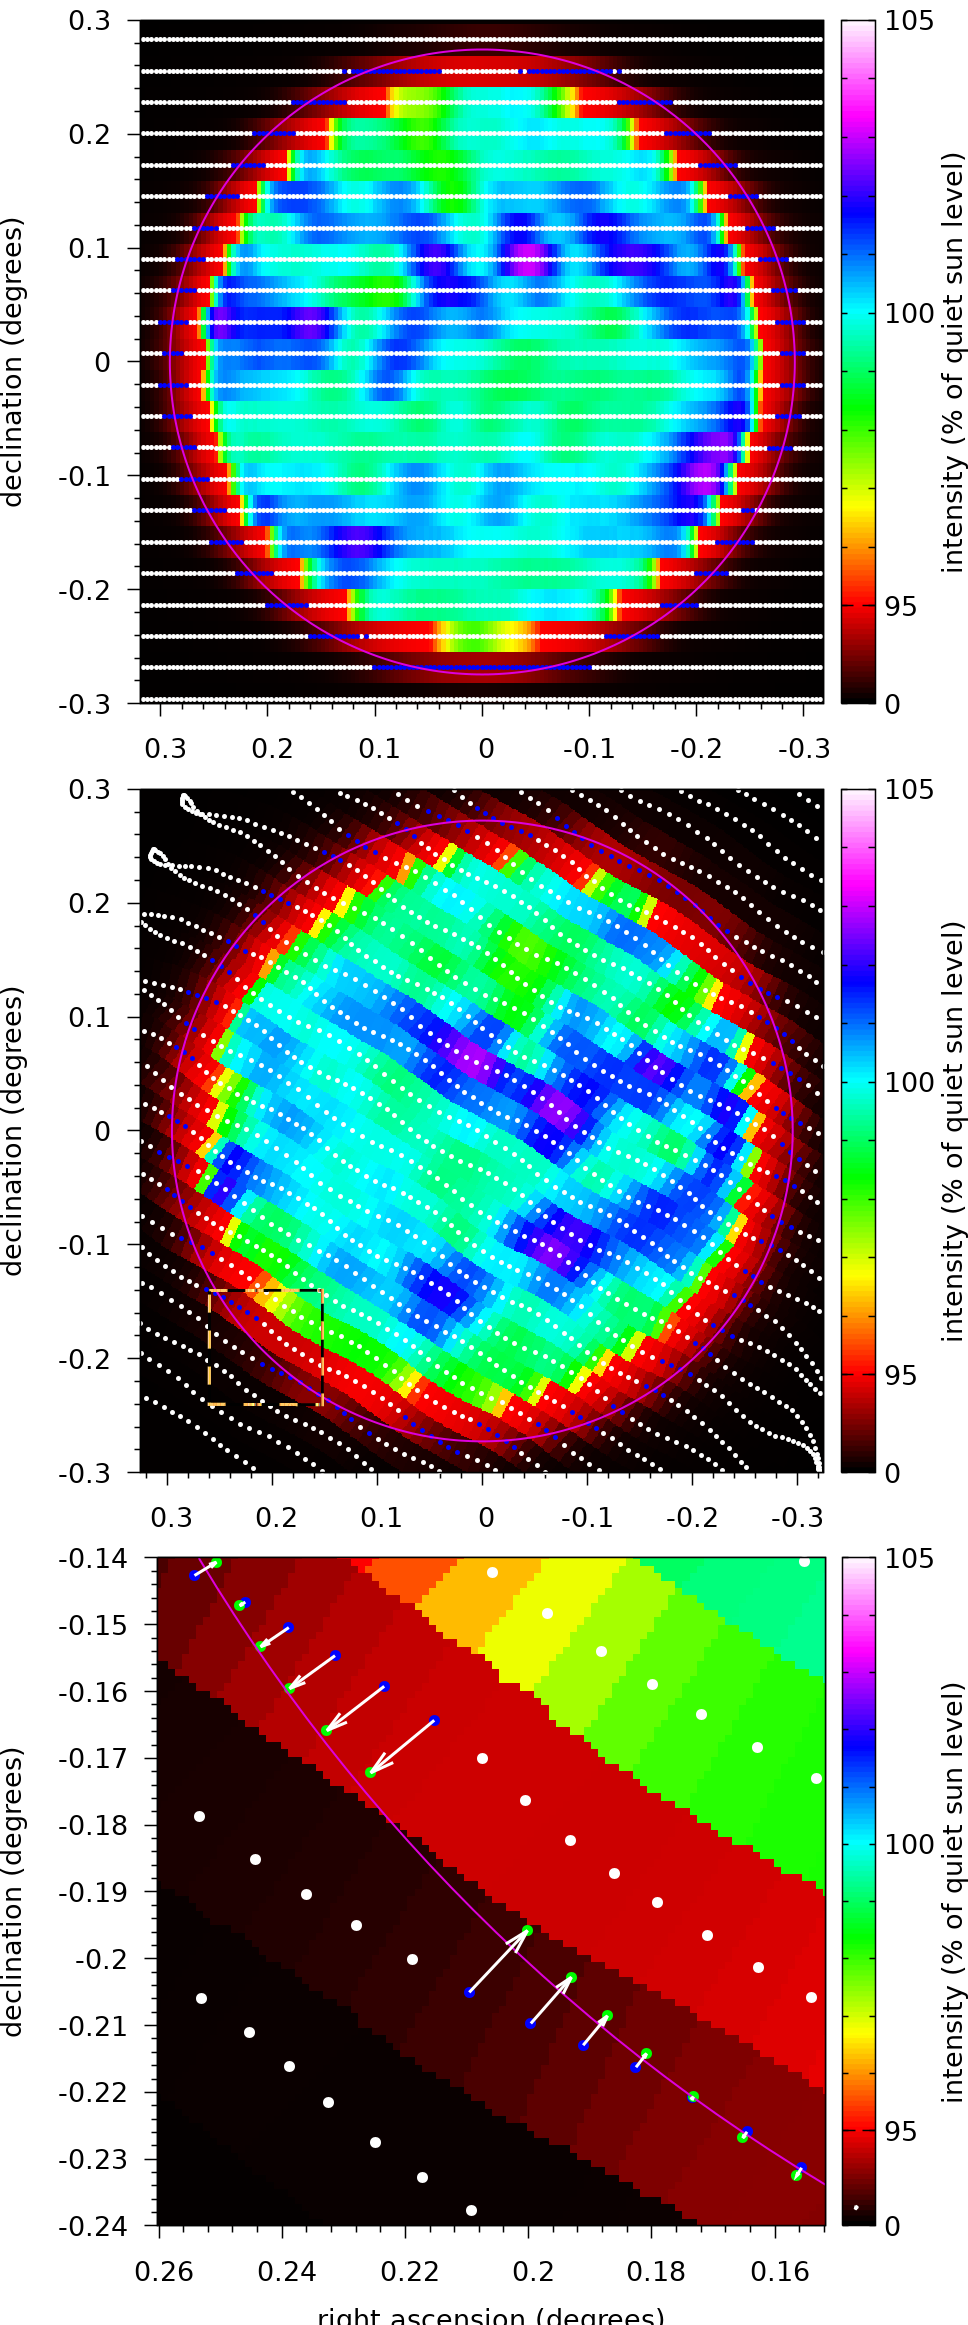
\includegraphics[width=\columnwidth]{nea_box.png}
  \begin{picture}(0,0)(0,0)
    \put(-85,608){\begin{large}\color{yellow}{\bf{(a)}}\end{large}}
    \put(-85,402){\begin{large}\color{yellow}{\bf{(b)}}\end{large}}
    \put(-85,200){\begin{large}\color{yellow}{\bf{(c)}}\end{large}}
  \end{picture}
  \caption{
    Typical Mets\"ahovi solar observations on $\SI{37}{GHz}$ {\bf(a)}
    25.07.2011 and {\bf(b)} 05.07.2016. Prior to May 2015 the observation beam
    scans along the equator, with samples mapped onto a rectangular grid.
    Since June 2015 a more accurate fit to the beam path was used, scanning
    horizontally. For the intensity color map each pixel is mapped to the
    nearest observed sample.
    This is an original uncalibrated map.
    {\bf(c)} Closeup of the 05.07.2016 map which 
    illustrates circle fitting.
    \fag{The x-axis label must be fully visible}
    \label{oldmap}\label{typicalmap}}
  \end{figure}
%------------------------------------------------------------------------------
Each line in a digital solar map file contains the time and coordinates of a sample as well as the recorded intensity 
value. The coordinates are relative to the expected location of the center of the Sun on the sky. The intensity is 
measured on $\SI{37}{GHz}$ and contains linear and logarithmic output from the amplifier as digital values. In this 
paper, we focus on the linear scale. However, the logarithmic scale is more sensitive for very low 
intensities and also avoids saturation during flare events, thus offering prospects for future 
research.

We use the word \emph{calibration} for describing the combined effort of normaliseing and centering a map. The applicable 
methods are described in Section\,\ref{sect:disk}. The raw intensities of a scan have an arbitrary scale, as in Fig.~\ref{typicalmap}{\bf(a-c)}. We 
need to normalise the signal levels and also correct for any minor offsets in the sample coordinates in order to have a 
properly centered map. The purpose of normalisation is to have zero intensity at the background and unit intensity for 
the QSL. For the contour maps up to year 1987, we trust the graphical markings and no calibration is needed.

\fag{Emphasis that A is new addition to previous published work. Made possible by Masters ...
and then clarify the distinction. What is new and how is our treatment new. C-B-A.}

%------------------------------------------------------------------------------
  \subsection{Disk fitting and signal levels} \label{sect:disk}

    
  %FAG: trying to disembiguate use of 'sample'
  %Each sample observation yields an intensity map with coordinates right 
  %Each observation scan yields an intensity map with coordinates right 
  %ascension, $\RA$, and declination, $\Dec$.
  %Each scan, denoted $S$ and spanning a couple of minutes, comprises a set of beam-size specimens. For $s_i \in S$:
  %FAG: trying to disembiguate use of 'sample'
  %SKK: maybe it could be clearer:
  Each solar map $S$ consists of $N_S$ samples $s_i$:
  \eqnl{radio_sample}{
    S &=& \left\{ s_i \;:\; i = 1, 2, ..., N_S \right\}\,\text{ and}\nonumber\\
    s_i &=& \left( t_i, x_i, y_i, u_i, ... \right),
  }
which specifies location $(x_i,y_i)$ and intensity $u_i$ as recorded at time
$t_i$ of each $s_i$ observation.
During calibration, as described below, additional derived quantities ($...$)
are attributed to each $s_i$.
Location is specified in equatorial coordinates relative to the expected
position, $(\RA_{\astrosun}, \Dec_{\astrosun})$, of the central point of Sun
at time $t_i$.
With right ascension cosine corrected, such that maps have unit aspect ratio, we apply 
\eqnl{relative_radec}{
  x_i = \frac{\RA(s_i)
      - \RA_{\astrosun}(t_i)}{\cos \left( \Dec_{\astrosun}(t_i) \right)}, &&
  y_i = \Dec(s_i) - \Dec_{\astrosun}(t_i)\text{.}
  }
  %FAG: rephrase
  %The absolute pointing of the antenna is not sufficiently accurate, while we can expect the relative accuracy to be 
  %better. We thus need to determine the center of the visual disk for each map. Also, since the signal levels $u_i$ are on arbitrary scale, we 
  %need to normalise them. A solar map consists of three regimes:
  We do not rely on the targeting accuracy of the antenna, and instead
  determine the center of the visual disk from each map $S$, from which we
  define the relative location of each $s_i$.
  Also, since the signal levels $u_i$ have arbitrary scale, 
  they need to be normalised.
  A map $S$ samples from each of the regions we designate as
  \begin{itemize}
  \item Background: The beam probes outer layers of the corona. Low intensity.
  \item Limb: Transition from corona to chromosphere.
  \item Disk: The beam probes chromosphere with varying incident angle. High intensity compared to background. Features, such as dim and bright regions, are visible.
  \end{itemize}

  For a map $S$, we will perform a preliminary statistical analysis (see Section~\ref{sect:s_curve}) in order to extract 
  two representative intensity values, $\s{u}{background}$ and $\s{u}{disk}$. We will then perform a linear 
  transformation for the raw intensity values $u_i$ and obtain the first normalized intensities $v_i^{(0)}$ as
  \eqnl{map_normalisation}{
  v_i^{(0)} := \frac{u_i - \s{u}{background})}{\s{u}{disk} - \s{u}{background}} \; \text{with} \; s_i \in S \text{.}
  }
  The normalized intensities are then used for initial centering of the map in Section~\ref{sect:initial-centering}. 
  This allows us to refine the equatorial coordinates of the samples as:
  \eqnl{map_centering}{
  \left( x_i^{(0)}, y_i^{(0)} \right) := \left( x_i, y_i \right) - \left( x^{(0)}, y^{(0)} \right) \text{.}
  }
  If the radius of the solar disk is not fixed, we can optionally also measure it. This finishes the initial calibration 
  round, for which we use a superscript $\cdot^{(c)}$ with $c=0$, also in Equations~\ref{map_normalisation} 
  and~\ref{map_centering}. This will be followed by additional calibration rounds, starting from 
  Section~\ref{sect:further_optimization}. Each calibration round produces a new normalized intensity value 
  $v^{(c+1)}$(Section~\ref{sect:disk_outliers}) for each sample. Using these new values $v^{(c+1)}$, the center for the 
  disk is further optimized as $(x^{(c+1)}, y^{(c+1)})$ in Section~\ref{sect:disk_outliers}.

  %FAG added
  %from which the initial radius of the disk, $r^(0)$, is estimated (Section~\ref{sect:initial_radius}). 
  %The superscript, 
  %(0), is used to indicate the initial values, which are then refined by an iterative process described in 
  %Sections~\ref{sect:iterative_calibration}, \ref{sect:outliers_disk} and \ref{sect:outliers_limb}. Following sufficient 
  %iterations we obtain calibrated maps $S^{(k)}$, from which we proceed to analyze and map the data onto heliographic 
  %coordinates and time series.
  %FAG: ended
  %\skk{There are no superscripts or subscripts for $S$. I have included the progressive calibration steps as additional 
  %values included in the bundles $s_i\in S$.}
  
  \subsubsection{Initial normalisation}\label{sect:s_curve}

  %FAG: rephrased
  %Sections~\ref{sect:s_curve} and~\ref{sect:initial-centering} describe the initial calibration step performed for the solar maps. This is based on an oral description 
  %given by Juha Aatrokoski at MRO, and a similar calibration method is commonly used at MRO.
  The initial normalisation and centering methods described here and in Section~\ref{sect:initial_centering} derive from 
  an oral outline given by Juha Aatrokoski at MRO of the calibration method commonly used at MRO, including 
  \citet{metsahovi40}.
  %\skk{Thanks Fred!}

  %FAG: removed para break and rephrase
  %In order to extract representatives $\s{u}{background}$ and $\s{u}{disk}$, we will first obtain a list of samples in 
  %map $S$, sorted by their raw intensity values $u_i$. Let $I_S$ be the set of indices for samples in $S$:

  In this step we initialise $\s{u}{background}$ and $\s{u}{disk}$. The samples in map $S$ are sorted by their raw 
  intensity values $u_i$. 
%\fg{I think this may be unnecessarily detailed (verbose). It can be summarised in words, 
%  alternative below...}i
 Let $I_S$ be the set of indices for samples in $S$:

%  \skk{Whether it is \emph{initialize} or \emph{initialise}, I think this time it is a thing which A\&A should decide.}

  \eqnl{S-curve_indices}{
  I_S = \left\{ 1, 2, ..., N_S \right\} \text{.}
  }
  We construct a monotonous integer function $w^{-1}$, such that
  $w^{-1}(j) = u_j$.
  The integer $j$ denotes the index of the re-ordered sample set $S = \left\{ s_j \right\}$ such
  that $j \le j^{\prime} \Leftrightarrow u_{j} \le u_{j^{\prime}}.$
  In Fig.~\ref{S-curve_example}{\bf(a)} , the inverse $w(u)$ is plotted against
  $u$ for a typical scan. For mathematical rigor, we need to handle the case of several samples having identical intensity:
  \eqnl{scurve-inverse-rigor}{
  w:\;\real \mapsto I_S, \quad w(u) = \max{0, j \in I_S:\; w^{-1}(j) \le u} \text{.}
  }

%  \skk{I included Fred's alternative wording but retained some of the formalism. I still need the index set $I_N$ later on.}

  %We are now free to choose the statistical functions $f$, $g$, $h$ which now describe the calibration algorithm. It is 
  %an open question whether we should use a fixed value for the visual radius, namely, should we fix $r_S = 
  %r_{\astrosun}(t_{\mathrm{mid},S})$. Radio frequency $\SI{37}{GHz}$ probes slightly higher altitudes compared to 
  %visible light, and we might thus expect a larger physical solar radius compared to $R_{\astrosun} = 6.957\times 10^8 
  %\mathrm{m}$. The standard value $R_{\astrosun}$ is based on visible light and optical depth of $\frac{2}{3}$. \skk{I 
  %have managed to produce an estimate $R_{\astrosun} = 7.10 \times 10^8 \mathrm{m}$ using an inversion model solver.}

  %We consider two disk methods to determine the solar disk position and size
  %from each map:
  %\begin{enumerate}
  %  \item $S$-curve and centre of mass: weighting the coordinates by the
  %  radio specimen intensity, $S$, center of mass.
  %  \item Convex hull: fitting a circle to those specimen coordinates, which
  %  we expect to belong to the solar limb, based on the geometry.
  %\end{enumerate}
  %We also consider three methods of signal level normalisation to identify
  %consistently between observations QSL and black sky:
  %\begin{enumerate}[a]
  %  \item  sort the intensity specimens and detect the point of zero curvature
  %  of the $S$-curve (specimen index vs. intensity).
  %  \fag{What is meant by constant fraction?}  
  %  \item iteratively calculate the statistical mean and standard deviation,
  %  excluding outliers, of the intensity of those points that are located
  %  within the solar disk and not too close to the limb.
  %  \item  detect two significant peaks from the intensity histogram,
  %  the lower intensity peak being the background and the higher the QSL.
  %\end{enumerate}
  %In this study, we present the optimal method combinations 1a, 2b and 2c.
%------------------------------------------------------------------------------

  \begin{figure}
  \centering
  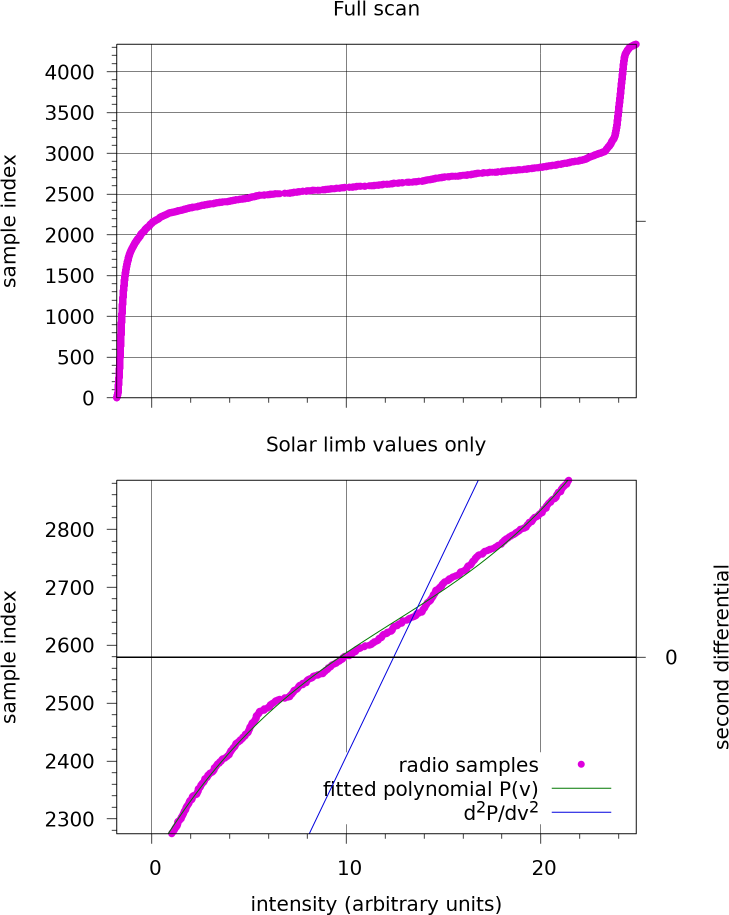
\includegraphics[width=8.5cm]{Scurve_example.png}
  \begin{picture}(0,0)(0,0)
    \put(-245,308){\begin{large}{\sf\bf{(a)}}\end{large}}
    \put(-245,146){\begin{large}{\sf\bf{(b)}}\end{large}}
  \end{picture}
  \caption{
    Radio samples of a typical solar scan sorted according to intensity.
    Panel {\bf(a)} displays all samples, with the limb transition between
    background and disk located with the dashed lines.
    A zoom in between the dashed line in {\bf(b)} includes the polynomial
    fit from Eq.~\eqref{scurve-approx}.
    A point of zero curvature (cross) provides a pivot point for signal level
    normalisation.}
  \label{S-curve_example}
  \end{figure}

  %central position. The data flow begins with radio intensity values $v_i$ measured on $\SI{37}{GHz}$ on time $t_i$ , 
  %right ascension $\mathrm{RA}_i$ and declination $\mathrm{dec}_i$. These equatorial coordinates are reported with respect 
  %to the known location of the Sun during the observation. Any analysis of the data is sensitive to the positioning of the 
  %solar disk, so instead of using the reported coordinates, they are first converted into a fitted coordinate system. Thus 
  %the size and location of the solar disk are determined from the data. Two complementary methods are used for measuring 
  %the center and size of the disk.
  
  Most samples belong either to the background or the disk. Both of these regimes constitute a narrow range of intensity 
  values and are observed as high slopes on $w(u)$. The limb region, however, contains more diverse intensity values and 
  produces a middle plateau in $w(u)$. We need an algorithm to define the exact center of this plateau for every map, and
  %MJK Limb samples only are shown in the lower panel, right? Please refer to the different panels appropriately.
  thus fit a sequence cubic (of degree $\s{n}{sc}=3$) polynomials $P_k$ such that:
  \eqnl{scurve-approx}{
  P_k(u) = \sum \limits_{n=0}^{\s{n}{sc}} a_n^{(k)} u^j \approx w(u) \text{.}
  }
  The fitting is performed as a quadratic optimization problem where we minimize the value of a target function $T_k$ over the domain $[\s{j}{min}^{(k)}, \s{j}{max}^{(k)}]$:
  \eqnl{scurve-target}{
  T_k(\bm{a}_k) = \sum \limits_{j = \s{j}{min}^{(k)}}^{\s{j}{max}^{(k)}} \left( w \left( w^{-1}(j) \right) - P_k \left( w^{-1}(j) \right) \right)^2 \text{.}
  }
  \fg{Perhaps most of the following details could be moved to an appendix and 
  here we just summarise the key points of the stage?}
  The domain of the first optimization round ($k=1$) contains the whole map:
  \eqnl{scurve-firstdomain}{
  \s{j}{min}^{(1)} := 1 \; \text{and} \; \s{j}{max}^{(1)} := N_S \text{,}
  }
  while the subsequent domain will be defined based on result of the previous optimization round. After obtaining 
  $P_k(u)$, we calculate the root $\s{u}{root}^{(k)}$, where the curvature of $P_k(u)$ changes from negative to 
  positive:
  \eqnl{scurve-root}{
  P_k^{\prime\prime}(\s{u}{root}^{(k)}) = 0 \implies \s{u}{root}^{(k)} = -\frac{a_2^{(k)}}{3 a_3^{(k)}} \text{.}
  }
  The root defines the pivot index for separating the disk from the background:
  \eqnl{scurve-pivot}{
  \s{j}{pivot}^{(k)} := P_k(\s{u}{root}^{(k)}) \text{.}
  }
  The representatives can now be assigned based on the pivot index as:
  \eqnl{scurve-background}{
  \s{u}{background}^{(k)} := w^{-1} \left( \floor{\frac{\s{j}{pivot}^{(k)} + 1}{2} + 0.5} \right) \text{and}
  }
  \eqnl{scurve-disk}{
  \s{u}{disk}^{(k)} := w^{-1} \left( \floor{\frac{\s{j}{pivot}^{(k)} + 2 N_S}{3} + 0.5} \right) \text{.}
  }
  The domain of the subsequent round is specified using the representatives:
  \eqnl{scurve-nextdomain-min}{
  \s{j}{min}^{(k+1)} := w \left( \floor{ 0.9 * \s{u}{background}^{(k)} + 0.1 * \s{u}{disk}^{(k)} + 0.5 } \right) \text{and}
  }
  \eqnl{scurve-nextdomain-max}{
  \s{j}{max}^{(k+1)} := w \left( \floor{ 0.1 * \s{u}{background}^{(k)} + 0.9 * \s{u}{disk}^{(k)} + 0.5 } \right) \text{.}
  }
  We then perform the next step $k := k+1$ and start by fitting a new polynomial in Equation~\ref{scurve-approx}. The 
  idea is that for the second round, we only use the limb samples and could expect a better fitting of $P_2$ compared to 
  $P_1$, while the $P_1$ already works well enough to find the plateau from full $w(u)$. The fitting in the second round is illustrated in Fig.~\ref{S-curve_example}{\bf(b)}.

  It is sufficient to stop the iteration at the second round and set:
  \eqnl{scurve-converged}{
  \s{u}{background} := \s{u}{background}^{(2)} \; \text{and} \; \s{u}{disk} := \s{u}{disk}^{(2)} \text{.}
  }
  It is also possible to use an odd order $n > 3$ for Equation~\ref{scurve-approx} and obtain slightly better precision 
  for the pivot $\s{i}{pivot}^{(k)}$. This leads to a failure if the resulting second differential $P_k^{\prime\prime}(u)$ 
  has zero or even number of real roots. Otherwise we can select the middle real root and proceed.

  \fg{Summarise the above and move the details to an appendix?}
  The initial normalised intensities $v_i^{(0)}$ can now be assigned using Equation~\ref{map_normalisation}.
  
  \subsubsection{Initial centering}\label{sect:initial_centering}

  For map $S$, we will calculate the weighted center of sample coordinates. For each sample $s_i \in S$ will be assigned an initial weight $b_i$:
  \eqnl{centering-initial-weight}{
  b_i^{(0)} := \begin{cases} 1 & \text{when}\; v_i^{(0)} \ge 0.85 \\ \frac{v_i^{(0)} - 0.15}{0.85 - 0.15} & \text{when}\; 0.15 < v_i^{(0)} < 0.85 \\ 0 & \text{when} v_i^{(0)} \le 0.15 \end{cases} \text{.}
  }
  Then center of mass is then:
  \eqnl{centering-center-of-mass}{
  \left( x^{(0)}, y^{(0)} \right) := \frac{\sum \limits_{i=1}^{N_S} b_i^{(0)} \left( x_i^{(0)}, y_i^{(0)} \right)}{\sum \limits_{i=1}^{N_S} b_i^{(0)}} \text{.}
  }
  This defines the initial center of the solar disk for the map, but it is further optimized below, starting from Section~\ref{sect:further_optimization}.

  \skk{Currenly, the code is not measuring the radius for each map. I implemented the functionality for 
  that, but probably we don't need it. If it turns out that the relative scale is inaccurate and varies between maps, we 
  can start using it. Maybe it would be clearer to omit the radius mode altogether. I just feel that it is relatively 
  easy to include the radius as a free parameter in case we so desire. If we think this as a methodology paper, the 
  radius measurement is a good bonus.}  
    \skk{I decided it is easier to convert the code into such form that it is easier to document, and the document it. 
    So now the S-curve -method and the calibration stuff described by J. Aatrokoski in MRO is used as an initiation step 
    for an iteration process. This iteration process selects limb samples a estimates they distance from the center. It 
    then fits a circle and neglects outliers. The centering is performed iteratively. I am almost done describing the 
    process thoroughly.}

    \skk{I though earlier about performing a comparison of the effectiviness of my convex hull method / limb model, the 
    S-curve method and the Shabasaki method. Actually these three methods are not completely overlapping in what they 
    perform, so they do not compete. And what I do is more iterative, and these two other methods only provide a 
    starting point for the iteration. Actually, I also wrote a simple method for producing a starting point, but the 
    S-curve method is more effective so I changed the code to use S-curve method first.}

    \skk{Anyway, the limb model -based iteration is what actually makes the centering.}
    
    \skk{There is another issue which I think is more serious. Metsähovi maps metadata are based on the standard value 
    for solar radius, $6.957 \times 10^8 \mathrm{m}$. For $\SI{8.1}{nm}$ wavelength, value $7.101 \times 10^8 
    \mathrm{m}$ is more realistic, based on \cite{Rozelot15}. By analyzing the Metsähovi maps I have managed to produce 
    two different values, based on different approaches. One, based on single day maps, produces $7.10 \times 10^8 
    \mathrm{m}$, which is pretty close. By using cycle 24 and a different definition for the radius, I arrive at $7.18 
    \times 10^8 \mathrm{m}$. I am currently reprosessing the data based on the later value of the radius.}
    
  \subsubsection{Initial radius}\label{sect:initial_radius}

  It is possible to calculate the radius of the disk as well. We start by calculating area integrals of a function $f(x,y) = x^2+y^2 = r^2$ over a disk of radius $R$, $\mathcal{B}(\bm{0},R)$. This gives:
  \eqnl{initial_radius}{
  Q = \int \limits_{(x,y) \in \mathcal{B}(\bm{0},R)} \! r^2 \dd x \dd y = \intef{r}{0}{R}{2 \pi r^3} = \frac{2 \pi}{4} \intes{r}{0}{R}{r^4} = \frac{\pi R^4}{2} \text{.}
  }
  The area of such a disk is $A = \pi R^2$. Thus the average value of $f(x,y)$ is:
  \eqnl{initial_radius2}{
  \ave f(x,y) = \frac{Q}{A} = \frac{R^2}{2} \text{.}
  }
  Following this reasoning, the initial radius of the disk on the map $S$ is:
  \eqnl{initial_radius3}{
  r^{(0)} := \sqrt{2 \frac{\sum \limits_{i=1}^{N_S} b_i^{(0)} \left( \left( x_i - x^{(0)} \right)^2 + \left( y_i - y^{(0)} \right)^2 \right)}{\sum \limits_{i=1}^{N_S} b_i^{(0)}}} \text{.}
  }
  Per map calibration of the radius is useful if the scale of the relative right ascension and declination would be inaccurate.

  In here we have assumed that the radius is known in advance, i.e. $r^{(c)} = r_{\astrosun}(t_S)$ for all calibration rounds $c$. Time $t_S$ is the middle time of scanning $S$, namely:
  \eqnl{initial_radius_time}{
  t_S = \frac{\min{t_i :\; s_i \in S} + \max{ t_i :\; s_i \in S}}{2} \text{.}
  }

  \subsubsection{Physical radius of the Sun}\label{sect:physical_radius}
  
  In this paper, we have assumed that the scale of the relative right ascension and declination are correct and thus the 
  radius of the disk is based on geometry. Let $R_{\astrosun}$ be the physical radius of the Sun and $d(t)$ be the distance 
  between MRO on Earth and the physical center (core) of the Sun at time $t$. Then:
  \eqnl{visual_angle}{
  r(t) = \arcsin \left( R_{\astrosun} / d(t) \right) \text{.}
  }
  The apparent radius of the Sun depends on wavelength and method of observation as well as the exact definition. For radio wavelengths, a quadratic fit 
  of the apparent radius $\ave r$ is constructed in \cite{Rozelot15}. Evaluating this for $\SI{37}{GHz}$ ($\lambda = 
  \SI{8.1}{mm}$ and the avarage distance of $\ave d = \SI{1}{AU}$, we obtain $R_{\astrosun} = 7.1006 \times 10^8 
  \mathrm{m}$.

  We have analyzed the solar radius using two different definitions which apply to MRO solar maps. Both definitions are 
  recursive and, by experience, shown to be convergent. They are described throughly in 
  Sections~\ref{sect:radius_method1} and~\ref{sect:radius_method2}. As for this paper we use the experimental value 
  $R_{\astrosun} = 7.176 \times 10^8 \mathrm{m}$ because it provides $0.5$ QSL intensity at the disk boundary.

  \subsubsection{Iterative calibration} \label{sect:further_optimization}

  Having obtained the initial ($c=0$) center of the disk as $(x^{(c)}, y^{(c)})$, and optionally, its radius $r^{(c)}$, we 
  proceed iteratively for $c:=c+1$. We accept the background intensity $\s{u}{background}$ from the initial calibration while perform 
  more analysis in order to determine the inner disk signal levels properly. We measure the QSL and its standard 
  deviation, while outliers within the disk are neglected. Between each QSL determination loop, we refine the centering 
  of the disk.
  
  \subsubsection{Inner disk outliers} \label{sect:disk_outliers}

  We aim to calculate the average intensity within the disk. However, we do not use the whole inner disk for measuring 
  QSL, since it typically contains bright and dim features such as active regions. These features will be neglected as 
  outliers in a series of iterative rounds.

  The beam pointing may be slightly 
  irregular due to oscillations in pointing. See Figure~\ref{typicalmap}{\bf(b)} for a typical antenna path. In 
  practice, the sweeps are moderately regular except for antenna wiggling, but our code does not expect uniform sample 
  density. We create a rectangular grid ($\Lambda$) of lattice points $\lambda_h \in \Lambda$. The lattice points are indexed via a set $I_{\Lambda}$:
  
  \eqnl{calib_inner_disk_lattice}{
  \Lambda = \left\{ \lambda_h :\; h \in I_{\Lambda} \right\} \text{.}
  }
  Each lattice point contains relative sky coordinates $\left( x_h, y_h \right)$ as well as an intensity value $u_h$:
  \eqnl{calib_inner_disk_point}{
  \lambda_h = \left( x_h, y_h, u_h \right) \text{.}
  }
  We can construct a lattice of desired integer resolution $\s{n}{grid} \in \mathds{N}$ by defining the index set as:
  \eqnl{calib_inner_disk_index}{
  I_{\Lambda} = \left\{ 0, 1, ..., \s{n}{grid}-1 \right\} \text{.}
  }
  We set up a rectangular frame to bound all the samples in $S$ as:
  \eqnl{calib_inner_disk_frame}{
  \s{x}{min} := \min{x_i:\, s_i \in S}, \; \s{x}{max} := \max{x_i:\, s_i \in S}, \; \s{y}{min} := \min{y_i:\, s_i \in S} \text{, and} \, \s{y}{max} := \max{y_i:\, s_i \in S} \text{.}
  }
  We define the index numbers as:
  \eqnl{calib_inner_disk_elem}{
  h = h_x \s{n}{grid} + h_y \; \text{where} \; 0 \le h_x,h_y < \s{n}{grid}, \; h_x,h_y \in \mathds{N} \text{.}
  }
  The coordinates are then obtained as:
  \eqnl{calib_inner_disk_lattice_x}{
  x_h := \s{x}{min} + \left( \s{x}{max} - \s{x}{min} \right) \frac{h_x}{\s{n}{grid}} \; \text{and}
  }
  \eqnl{calib_inner_disk_lattice_y}{
  y_h := \s{y}{min} + \left( \s{y}{max} - \s{y}{min} \right) \frac{h_y}{\s{n}{grid}} \text{.}
  }
  The intensity associated with a lattice point $\lambda_h$ is that of the nearest sample $s_i \in S$, which is obtained via mapping $i_{\Lambda}:\; I_{\Lambda} \mapsto I_S$:
  \eqnl{calib_inner_disk_lattice_u}{
  u_h := u_i, \; i = i_{\Lambda}(h) \text{.}
  }
  The mapping $i_{\Lambda}(h)$ transforms the lattice point of index $h$ into the map sample of index $i$, so that the nearest sample is chosen. The distance between $\lambda_h$ and $s_i$ is measured as $d_h$ using uncalibrated coordinates:
  \eqnl{calib_inner_disk_nearest1}{
  d_h^2 = \min{\left( x_i - x_h \right)^2 + \left( y_i - y_h \right)^2:\; s_i \in S} \; \text{and}
  }
  \eqnl{calib_inner_disk_nearest2}{
  \left( x_{i_{\Lambda}(h)} - x_h \right)^2 + \left( y_{i_{\Lambda}(h)} - y_h \right)^2 = d_h^2 \text{.}
  }
   When several map samples satisfy Equation~\ref{calib_inner_disk_nearest2}, the mapping $i_{\Lambda}(h)$ is chosen 
  arbitrarily. It is possible to use e.g. linear interpolation based on Voronoi tessellation here. However, currently it 
  is not implemented. \skk{I wanted to implement Voronoi tessellation but the code has already grown to have too many 
  features that it was not feasible. Currently I am working with the inversion model solver, which has no need for any 
  interpolation anyway. So writing the tessellation ready is still possible but a side step to my opinion, and that is 
  why I gave up.}
 
  For each calibration round $c$, we define the inner disk $I_c \subset \Lambda$ as the region that is within $0.9 r^{(c)}$ distance from origin, using centered coordinates:
  \eqnl{calib_inner_disk1}{
  I_c := \left\{ \lambda_h :\; \sqrt{\left( x_h - x^{(c)} \right)^2 + \left( y_h - y^{(c)} \right)^2} \le 0.9 r^{(c)} \right\} \text{.}
  }  
  For first outlier neglection round, we have $q=0$ and set $I_{c}^{(0)} := I_c$. We calculate the average intensity $\s{u}{QSL}^{(c,q)}$ and standard deviation $\s{\sigma}{QSL}^{(c,q)}$ as follows:
  \eqnl{calib_inner_disk2}{
  \s{u}{QSL}^{(c,q)} := \frac{1}{|I_{c}^{(q)}|} \sum \limits_{\lambda_h \in I_{c}^{(q)}} u_h \; \text{and}
  }
  \eqnl{calib_inner_disk3}{
  \s{\sigma}{QSL}^{(c,q)} := \sqrt{\frac{1}{|I_{c}^{(q)}|} \sum \limits_{\lambda_h \in I_{c}^{(q)}} \left( u_h - \s{u}{QSL}^{(c,q)} \right)^2} \text{.}
  }
  The subsequent outlier neglection rounds omit the lattice points whose intensities are not within two standard deviations from the average, when previous outliers are neglected:
  \eqnl{calib_inner_disk4}{
  I_c^{(q+1)} := \left\{ \lambda_h \in I_c^{(q)} :\; \left|u_h^{(c)} - \s{u}{QSL}^{(c,q)} \right| \le 2 \s{\sigma}{QSL}^{(c,q)} \right\} \text{.}
  }
  After a few rounds, $q = \s{q}{max}$, the set of non-outliers converges and we have obtained a new reference 
  intensity. We can now define the QSL and its standard deviation for the next calibration round $c \mapsto c+1$ as:
  \eqnl{calib_inner_disk5}{
  I_{c+1}^{(\mathrm{QSL})} := I_{c}^{(\s{q}{max}+1)},\; \s{u}{QSL}^{(c+1)} := \s{u}{QSL}^{(c,\s{q}{max})} \text{, and} \; \s{\sigma}{QSL}^{(c+1)} := \s{\sigma}{QSL}^{(c,\s{q}{max})} \text{.}
  }
  For the next calibration round, the sample intensities are renormalized:
  \eqnl{calib_inner_disk6}{
  v_i^{(c+1)} := \frac{u_i - \s{u}{background}}{\s{u}{QSL}^{(c+1)} - \s{u}{background}} \text{.}
  }
  The first time we run the above substitions (Section~\ref{sect:disk_outliers}) is for $c=0$.

  \subsubsection{Bright and dim features} \label{sect:bright_dim_features}

  From now on, the first round is for $c=1$. We separate the inner disk of the previous centering round, $I_{c-1}$, into three subsets, 
  $I_c^{(\mathrm{dim})}$, $I_c^{(\mathrm{QSL})} = I_{c-1}^{(\s{q}{max}+1)}$, and $I_c^{(\mathrm{bright})}$ based on 
  normalized signal levels:
  \eqnl{calib_features_dim}{
  I_c^{(\mathrm{dim})} := \left\{ \lambda_h \in I_{c-1} :\; u_h - \s{u}{QSL}^{(c)} < -2 \s{\sigma}{QSL}^{(c)} \right\} \; \text{and}
  } 
  \eqnl{calib_features_bright}{
  I_c^{(\mathrm{bright})} := \left\{ \lambda_h \in I_{c-1} :\; u_h - \s{u}{QSL}^{(c)} > 02 \s{\sigma}{QSL}^{(c)} \right\} \text{.}
  } 
  We will partition the lattice points in $I_c^{(\mathrm{dim})}$ and $I_c^{(\mathrm{bright})}$ into a set of features $\mathcal{F}_c$ such that:
  \eqnl{calib_features2}{
  \bigcup \limits_{F \in \mathcal{F}_c} F = I_c^{(\mathrm{dim})} \cup I_c^{(\mathrm{bright})} \text{.}
  }
  Any two features $F, F^{\prime} \in \mathcal{F}_c$, $F \ne F^{\prime}$ are separate such that $F \cap F^{\prime} = 
  \emptyset$. Any two neighbouring lattice points $\lambda_h, \lambda_{h^{\prime}} \in I_c$ satisfy the clustering 
  requirement. If either $\lambda_h,\lambda_{h^{\prime}} \in I_c^{(\mathrm{dim})}$ or $\lambda_h,\lambda_{h^{\prime}} 
  \in I_c^{(\mathrm{bright})}$, then there is a feature $F \in \mathcal{F}_c$ such that $\lambda_h,\lambda_{h^{\prime}} 
  \in F$. Thus any connected bright or dim pattern on the solar disk, significantly outside the range of the QSL 
  intensitities, will constitute a feature $F \in \mathcal{F}_c$. The features are typically bright and dim regions on 
  chromosphere, but they can also arise from instrumental effects just as changing weather conditions during observation 
  of $S$.
  
  The area of a feature $F$, $A(F)$, is the number of lattice points in $F$ times the lattice square area:
  \eqnl{calib_features3}{
  A(F) := |F| \frac{\left( \s{x}{max} - \s{x}{min} \right) \left( \s{y}{max} - \s{x}{min} \right)}{\s{n}{grid}^2} \text{.}
  }
  We define the radius $r(F)$ of a feature $F$ as the radius of circle which has area $2 A(F)$:
  \eqnl{calib_features4}{
  r(F) := \sqrt{\frac{2 A(F)}{\pi}} \text{.}
  }
  The location $z(F)$ of a feature $F \in \mathcal{F}_c$ is calculated as a center of mass using calibrated coordinates and QSL relative intensity as weight:
  \eqnl{calib_features5}{
  z(F) := \left( x(F), y(F) \right) = \frac{\sum \limits_{\lambda_h \in F} \left( x_h, y_h \right) \left| u_h - \s{u}{QSL}^{(c)} \right|}{\sum \limits_{\lambda_h \in F} \left| u_h - \s{u}{QSL}^{(c)} \right|} - \left( x^{(c-1)}, y^{(c-1)} \right) \text{.}
  }

  \subsubsection{Limb outliers} \label{sect:outliers_limb}

  In the next step of this algorithm, we will neglect those antenna samples which are too close to any known feature. We form a set $L^{(c)}_1 \subset S$ based on Equation~\ref{calib_features5}.
  \eqnl{calib_features6}{
  L^{(c)}_1 := S \setminus \bigcup \limits_{F \in \mathcal{F}_c} \left\{ s_i \in S: \; \sqrt{\left( x^{(c-1)}_i - x(F) \right)^2 + \left( y^{(c-1)}_i - y(F) \right)^2} \le r(F) \right\} \text{.}
  }
  We will calculate a relative radial distance for each sample $s_i \in S$ based on previous round $c-1$:
  \eqnl{calib_radial_distance}{
  r_i^{(c)} := \frac{\sqrt{\left( x_i - x^{(c-1)} \right)^2 + \left( y_i - y^{(c-1)} \right)^2}}{r^{(c-1)}} \text{.}
  }
  For detecting limb outliers, we collect a subset $L^{(c)}_2 \subset S$ of the map $S$ which restricts radial distances into the boundary region:
  \eqnl{calib_subset1}{
  L^{(c)}_2 := \left\{ s_i \in S:\; 0.96 \le r_i^{(c)} \le 1.04 \right\} \text{.}
  }
  These points reside at the limb when it comes to the current centering round $c$. Further requirement for the limb is that the intensities must also be consistent with being on the limb, defining another subset.
  \eqnl{calib_subset2}{
  L^{(c)}_3 := \left\{ s_i \in S:\; 0.05 \le v_i^{(c)} \le 0.95 \right\} \text{.}
  }
  The final boundary set $L^{(c)}$ is taken as:
  \eqnl{calib_subset3}{
  L^{(c)} := L^{(c)}_1 \cap L^{(c)}_2 \cap L^{(c)}_3 \text{.}
  }
  We thus want to avoid any known chromospheric features when they are close to the limb, since they would produce 
  exceptional values there and interfere with proper centering. Having obtained $L^{(c)}$, we calculate a radial 
  estimate: $r_i^{\prime(c)}$, for each $s_i \in L^{(c)}$. This is based on a known limb profile $l_{p,S}(r)$. For details on how the 
  limb model is obtained, please refer to Section \ref{sect:radius_method1}. Initially, we had no forehand details of 
  the limb and the model had to be constructed using more rudimentary methods. Another option for bootstrapping is to assume a simple linear function for the first limb model round $p=0$:
  \eqnl{calib_limbmodel1}{
  l_{0,S}(r) = \frac{1.04 - r}{1.04 - 0.96} \text{.}
  }
  After maps of a given solar cycle have been processed, we can construct a more sophisticated limb model for the next grand iteration round $p := p+1$. First we need 
  to optimize the target in Equation~\ref{physical_radius_target} and obtain parameters for functions in 
  Equation~\ref{physical_radius_polynomials}. Denote $a_S = a_{\astrosun}(t_S)$ for the altitude where the center of the Sun is as seen from 
  MRO during observation of map $S$. The limb model for $S$ at round $p \ge 1$ is 
  then:
  \eqnl{calib_limbmodel2}{
  l_{p,S}(r) = \frac{B(\bm{x}_m^{(p)}, \rho(r), a_S)}{B(\bm{x}_m^{(p)}, \rho(1/3), a_S)} \text{.}
  }
  The parameter set $\bm{x}_m^{(p)}$ is optimized for round $p$ and with sufficiently large $m$. Figure~\ref{limb_brightening} illustrates the optimized limb profiles of cycle 24 for the applicable range of altitudes.
  The radial estimate is obtained from the inverse of $l_{p,S}(r)$ as:
  \eqnl{calib_limbmodel3}{
  l_{p,S}(r_i^{\prime(c)}) = v_i^{(k)} \implies r_i^{\prime(c)} := l_{p,S}^{-1}(v_i^{(c)}) \text{.}
  }

%------------------------------------------------------------------------------
\begin{figure}
\centering
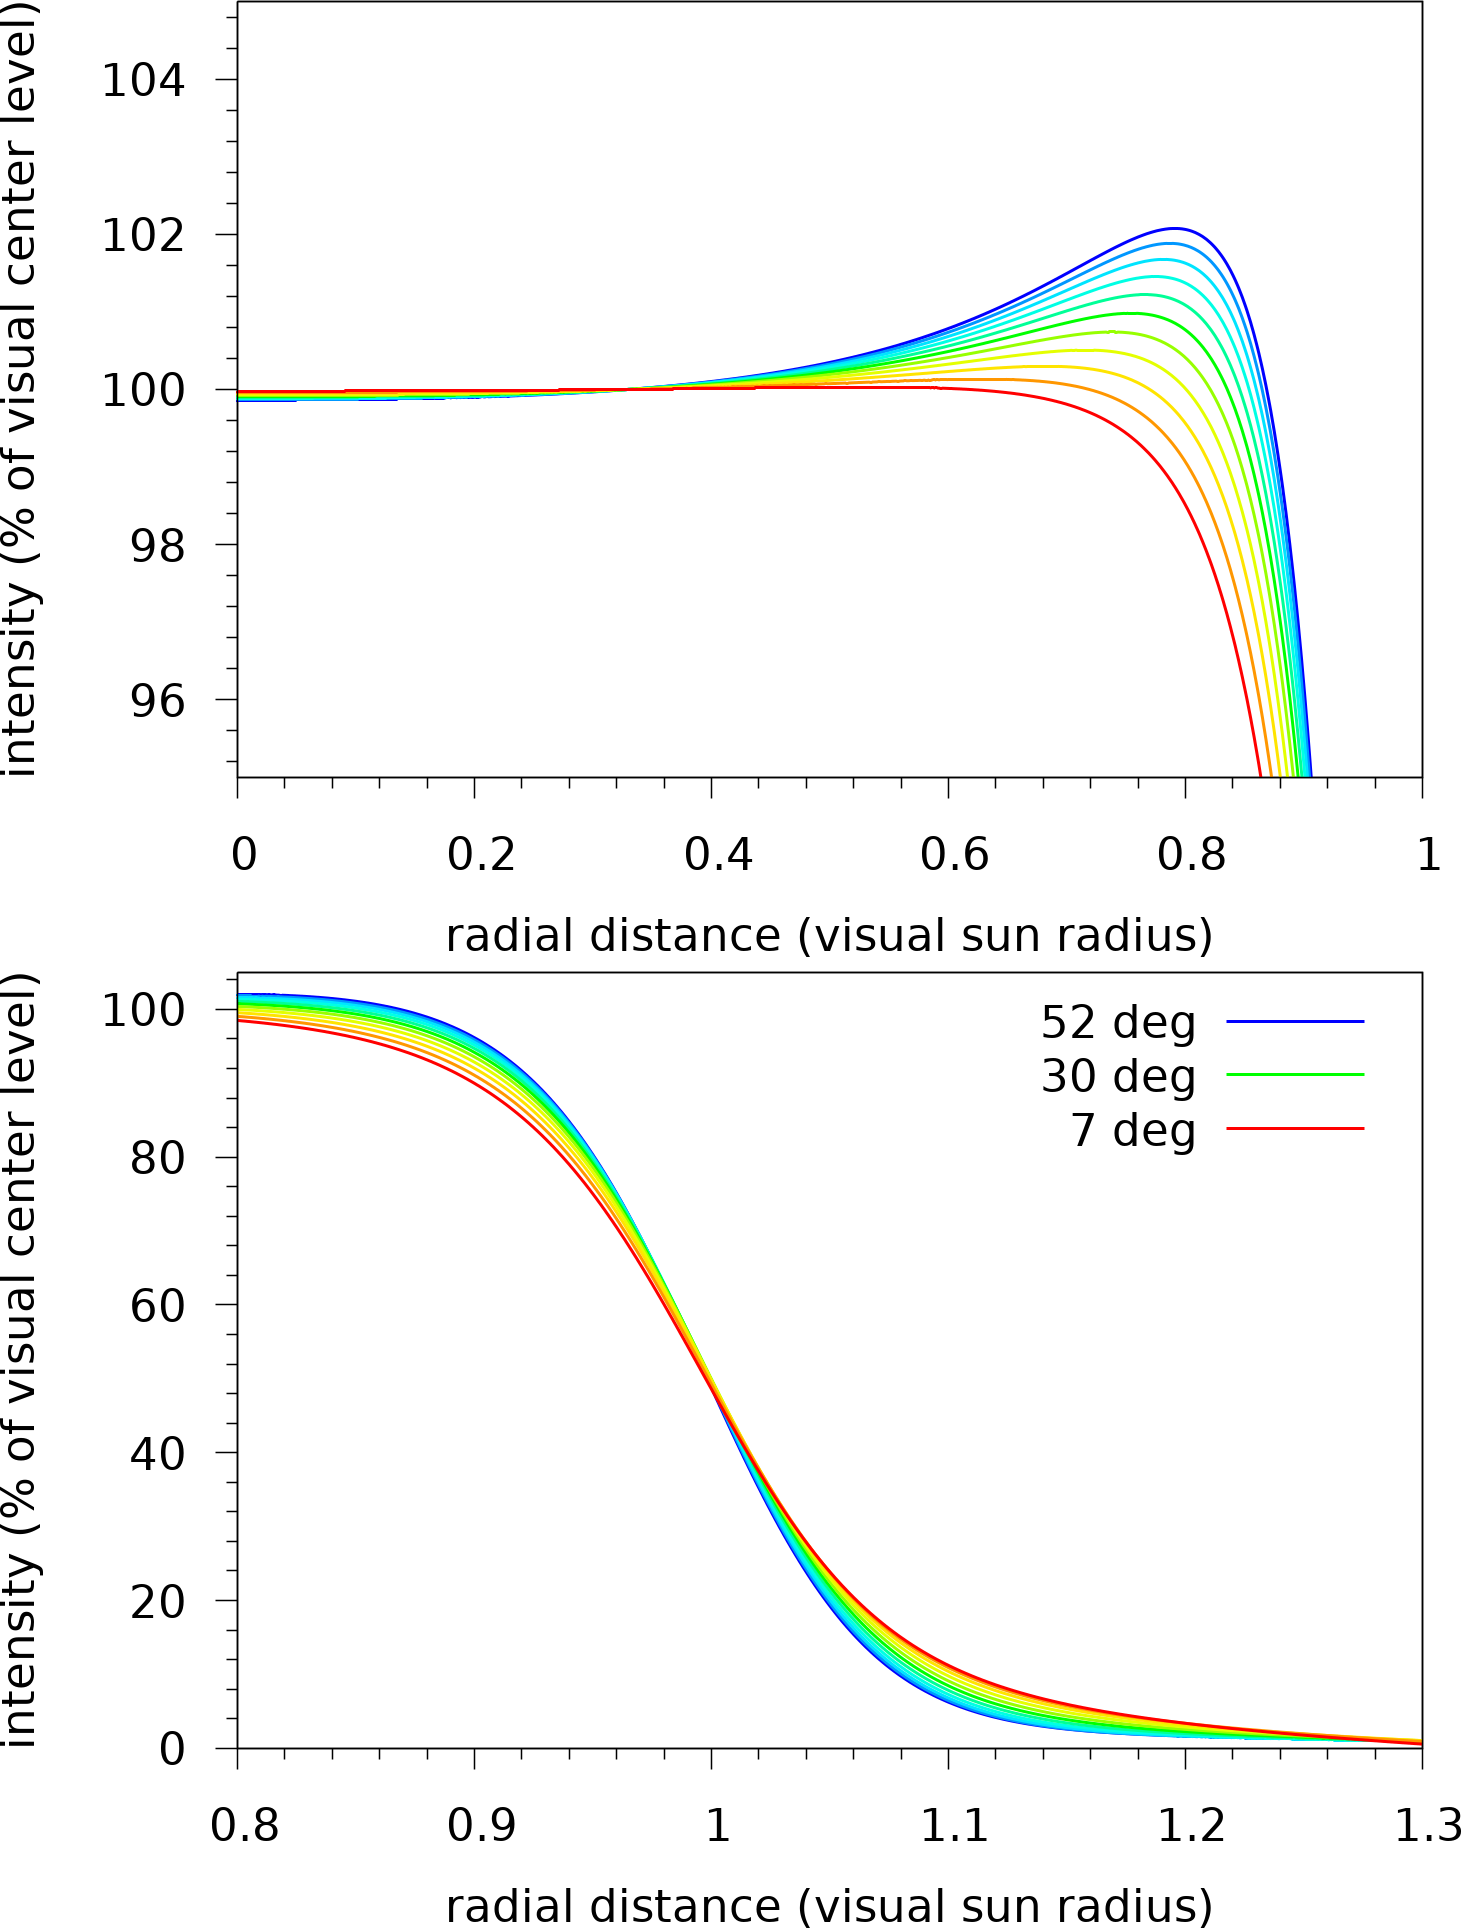
\includegraphics[width=8.5cm]{limbmodel_profiles.png}
  \begin{picture}(0,0)(0,0)
    \put(-205,306){\begin{large}{\sf\bf{(a)}}\end{large}}
    \put(-205,146){\begin{large}{\sf\bf{(b)}}\end{large}}
  \end{picture}
%\begin{picture}(0,0)(0,0) \put(-220,315){\begin{huge}a\end{huge}} \put(-220,158){\begin{huge}b\end{huge}} \end{picture}
\caption{Average quiet Sun intensity as a function of radial distance from the visual center, normalised for the intensity at $0.33$ radii from the center. a) Limb brightening is observed when line of sight is almost tangential to the solar surface. b) The beam 
size of $2.4^\prime$ mixes the solar limb with the dark background, resulting in a convolution pattern. On both plots, we observe more blurring when the altitude of observation is low, due to atmospheric effects.}
\label{limb_brightening}
\end{figure}
%------------------------------------------------------------------------------
  
  The radial error for each sample $s_i$ is then calculated as difference between the real and estimated radius:
  \eqnl{calib_deviation1}{
  \delta r_i^{(c)} := r_i^{(c)} - r_i^{\prime(c)} \text{.}
  }
   We want to neglect outliers for which the radial error is too high. These are associated with activity on the limb or 
  a with an instrumetal error. The outlier filtering is done iteratively, starting with $g=4$ and setting $L^{(c)}_4 := 
  L^{(c)}$.
  For a given set of limb samples, $L^{(c)}_g$, we can calculate the standard deviation of radial estimates as:
  \eqnl{calib_deviation2}{
  \Delta \left( L^{(c)}_g \right) = \sqrt{\frac{\sum \limits_{s_i \in L^{(c)}_g} \left( \delta r_i^{(c)} \right)^2}{\left|L^{(c)}_g \right|}} \text{.}
  }
  The subsequent boundary sets $g \mapsto g+1$ are constructed from $L^{(c)}$ as follows:
  \eqnl{calib_deviation3}{
  L^{(c)}_{g+1} = \left\{ s_i \in L^{(c)} : \; \left|\delta r_i^{(c)} \right| \le 2 \Delta \left( L^{(c)}_{g} \right) \right\} \text{.}
  }
  After a couple of steps we have neglected any outliers with good reliability. We can use the limb set $L^{(c)}_{\s{g}{out}}$ with $\s{g}{out} := 10$for this.

  \subsubsection{Subsequent centering} \label{sect:subsequent_centering}

  We will fit a circle into the set $L^{(c)}_{\s{g}{out}}$. The quality of fitting is evaluated as $T_c$:
  \eqnl{subsequent_centering1}{
  T_c(\bm{z}) = \sum \limits_{s_i \in L^{(c)}_{\s{g}{out}}} \left( \sqrt{\left( x_i - x \right)^2 + \left( y_i - y \right)^2} - r_i^{(c)} r \right)^2 \text{.}
  }
  Here the vector $\bm{z} = \left( x, y, r \right)^T$.
  The radius $r$ is optionally a free parameter, otherwise we fix $r := r^{(c)} = r^{(0)}$ (see 
  Section~\ref{sect:initial_radius}). We search of optimal values $\bm{z}_{\zeta}^{(c)}$ which minimize $T_c$, starting with $\zeta=0$:
  \eqnl{subsequent_centering2}{
  \bm{z}_0^{(c)} := \left( x^{(c-1)}, y^{(c-1)}, r^{(c-1)} \right)^T \text{.}
  }
  We assume that $T_c(\bm{z})$ is locally quadratic with $H_c(\bm{z})$ begin the Hessian of $T_c(\bm{z})$:
  \eqnl{subsequent_centering3}{
  T_c(\bm{z}+\delta \bm{z}) \approx T_c(\bm{z}) + \delta \bm{z}^T \nabla T_c(\bm{z}) + \frac{1}{2} \delta \bm{z}^T H_c(\bm{z}) \delta \bm{z} \text{.}
  }
  The quadratic approximation has minimum at: $\delta \bm{z} = -H_c^{-1}(\bm{z}) \nabla T_c(\bm{z})$. By iterating as:
  \eqnl{subsequent_centering4}{
  \bm{z}_{\zeta+1} := \bm{z}_{\zeta} - H_c^{-1}(\bm{z}_{\zeta}) \nabla T_c(\bm{z}_{\zeta}) \text{,}
  }
  we arrive at a true minimum of $T_c$ in few steps. The convergence is detected when the value of $T_c$ no longer 
  decreases in subsequent iterations due to numerical limits and small shift $\delta \bm{z}_{\zeta}$. This optimum value defines the new center and radius for the map:
  \eqnl{subsequent_centering5}{
  \left( x^{(c)}, y^{(c)}, r^{(c)} \right)^T := \lim \limits_{\zeta \to \infty} \bm{z}_{\zeta} \text{.}
  }
  We will now loop back to Section~\ref{sect:outliers_disk} unless we have reached $c = \s{c}{max} := 5$. \skk{Hey, natural language is also a programming language.}
  In subsequent sections, we will use the fully calibrated values $x_i^{(\s{c}{max})}$, $y_i^{(\s{c}{max})}$, and $r_i^{(\s{c}{max})}$ for each sample $s_i \in S$.

\skk{Moved the convex hull stuff into a separate file, probably not to be included in the paper.}

%------------------------------------------------------------------------------
\subsection{Limb correction model}\label{sect:limb}

%FAG rephrase
%We intend to estimate the brightness ($v$) based on time ($t$), heliographic latitude ($\theta$), angular distance from the 
%%MJK comma '...disk, as seen...'
%center of solar disk as seen at the time of observation ($r$), and the altitude above the horizon ($\varphi$). The model 
%will contain polynomials of high degree, so that numerical stability is a concern. We need to carefully select the 
%domains for each parameter. Radians are a natural choice of units for $\theta, \varphi \in \left( 0, \frac{\pi}{2} 
We seek to determine the brightness ($v$) at time ($t$), heliographic latitude
($\theta$) and angular distance from the centre of solar disk, based on an
%FAG we introduce r here, but do not appear to use it and can confuse with radius
%FAG: does it refer to the observation time or the observation as a specimen?
observation at time ($\tau$) and altitude above the horizon ($\varphi$).
We model with polynomials of high degree, so care with numerical stability is 
required, matching separately domains for each parameter.
Radians are a natural choice of units for $\theta, \varphi \in \left( 0, \pi/2 
%FAG reformat
%\right)$. For time, $t = \frac{a - 2005}{10}$, where $a$ is a real number $a = 1970 + 
%\frac{\mathrm{unixtime}}{60\cdot60\cdot24\cdot365.25}$. Radius $r$ is represented as relative to the visual solar radius, which can 
%either be calculated from our astronomical model or fitted to the data as a circle.
\right)$. For time, $t = (a - 2005)/10$, where $a$ is a real number $a = 1970 +
\mathrm{unixtime}/(60\cdot60\cdot24\cdot365.25)$. Radius $r$ is represented as
%FAG: sami is this correct reference to methods
relative to the visual solar radius, which can be calculated either from our
astronomical model (method 1) or fitted to the data as a circle (method 2).

%FAG. is this a repeat of 2.2
The solar map is a collection of intensity values $\left\{ v_i \right\}_i$ 
sampled by the antenna.
These are linearly scaled so that $1$ represents the QSL and $0$ represents
the black sky.
Each intensity value $v_i$ is accompanied with right ascension $\delta \mathrm{RA}_i$ and declination $\delta 
\mathrm{dec}_i$relative to the center of the solar disk, $\left( \mathrm{RA}_{\mathrm{sun}}(t_i), 
\mathrm{dec}_{\mathrm{sun}}(t_i) \right)$, at the time of observation, $t_i$.


Moreover, $\varphi_i$ will be the altitude of the solar center at the time of observation, relative 
to observers horizon. It is measured in radians, and in practice samples will have the range:
\eqnl{altitude_range}{
\varphi_i \in \left[ \frac{5}{180} \pi, \frac{53}{180} \pi \right] \text{.}
}
%FAG added reference to Fig 3 and para break. Sami is this correct and an
%FAG appropriate place to mention the Fig?
In Fig.\,\ref{limb_brightening}(a), we show the effect of limb brightening for
observations within the range $\varphi_i\in[7\deg,52\deg]$, and in
Fig.\,\ref{limb_brightening}(b) the corresponding correction profiles, which 
are applied near the limb to compensate.

%FAG: moving to results where creating the butterfly maps will now be discussed
%Each sample also has weight $w_i$, which is set as to balance the target set. 
%There are more 
%observations starting from year $2015$, while only a few maps for year $1989$. 
%%MJK Often we do just the opposite: if there are less data for a certain epoch, then the weigth is lower because of that time interval in more uncertain. Please expand on the logic here.
%Thus we will put more weight on the old 
%maps. Summer days typically have dozens of maps as the observational day is long, while on winter there are only a few maps per day.
%
%We get more samples from the low heliographic latitudes, since a greater length of the solar equator is visible, 
%compared to high latitude arcs. During summer, the solar north pole is visible to Earth, while we also get observations 
%from high altitudes. During winter, we only observe the Sun at low altitude, and the solar south pole is visible. 
%Further investigations are needed to exclude any bias effects arising from the unbalanced target set. However, having 
%separate polynomials $P_n$ and $Q_m$ should reduce these risks. 
%%MJK Good idea, but sounds like a task not necessary to undertake now? If the referee asks us to verify this risk, then we should do it. But, I comment it out for now...
%%I suggest testing the optimization code with simulated 
%%data.
%
%%MJK The active region tracking tool is not yet described here. You are still planning to include that, right?
%
%Limb intensity profiles showing brightening. 

%------------------------------------------------------------------------------
\subsection{Heliographic coordinates from radio data}\label{sect:helio}




%A particular radio data sample $s_i$ contains time $t_i$, relative position on the sky $(\delta \mathrm{RA}_i, \delta 
%\mathrm{dec}_i$), and measured intensity $u_i$in arbitrary linear units. For convenience, we use two equivalent 
%conventions for sample notation:
%
%%MJK Introducing line break to fit the equations on a single line
%%\eqnl{radio_sample}{
%%s_i = \left( t_i, \delta \mathrm{RA}_i, \delta \mathrm{dec}_i, u_i \right) = \left( t(s_i),\delta \mathrm{RA}(s_i), \delta \mathrm{dec}(s_i), u(s_i) \right) \text{.}
%%}
%\eqnl{radio_sample}{
%s_i &=& 
%\left( t_i, \delta \mathrm{RA}_i, \delta \mathrm{dec}_i, u_i \right) \\ \nonumber
%&=& \left( t(s_i),\delta \mathrm{RA}(s_i), \delta \mathrm{dec}(s_i), u(s_i) \right) \text{.}
%}
%%Observation is done at time $t_i$ and from geographic location 
%%$(\phi_{\earth}, \lambda_{\earth}) = \left( +60.217797339^{\circ}, +24.393084663 \right)$, which is 
%%Metsähovi Radio Observatory.
%Each scan $S = \left\{ s_i \right\}_{i=\s{i}{min}}^{\s{i}{max}}$ consists of maps taken 
%during $\s{t}{min}(S) \le s_i \le \s{t}{max}(S), \; s_i \in S$.
%The equatorial coordinates used are relative to the expected position of the central point
%of the Sun at $t_i$ and they are cosine corrected to have unit aspect ratio:
%\eqnl{relative_radec}{
%\delta \mathrm{RA}_i  &=& \frac{\mathrm{RA}_i - \mathrm{RA}^{\astrosun}(t_i)}{\cos \left( \mathrm{dec}^{\astrosun}(t_i) \right)} \\
%\delta \mathrm{dec}_i &=& \mathrm{dec}_i - \mathrm{dec}^{\astrosun}(t_i) \text{.}
%}
%In this work, we study only samples taken on $\SI{37}{GHz}$.
%The raw intensity $u_i$ is measured in arbitrary units.
Our solar maps are not sensitive to small systematic pointing errors or inter map variations in signal levels, since we calibrate each scan individually.
% determine the position and size of the solar disk as well as signal levels in the background and within the quiet sun area.
%MJK not to confuse the reader, refer already forward
We apply algorithm $F_j$,
%MJK
defined in detail in Sect.~\ref{sect:disk},
%MJK
for the scan $S$ in order to produce a disk model:
\eqnl{disk_model}{
F_j(S) = \left( \delta \mathrm{RA}_S, \delta \mathrm{dec}_S, r_S, \s{u}{background}(S), \s{u}{QSL}(S) \right) \text{.}
}
%The disk fitting model in $F_j$ is used for correcting small tracking errors and calibrating the intensity levels.
We then obtain calibrated position and intensity for each sample. Signal levels are scaled so that zero is for the background and unity for the 
%MJK OK, defined here, hence:
%Quiet Sun Level (QSL):
QSL:
%\eqnl{calibrated_samples}{
%c_i = F(S)(s_i) = \left( t_i, x_i, y_i, v_i \right) \text{,}
%}
%such that:
\eqnl{calibration}{
x_i &=& \frac{r^{\astrosun} \left( \s{t}{mid}(S) \right)}{r_S} \left( \mathrm{RA}_i -  \mathrm{RA}_S  \right) \\
y_i &=& \frac{r^{\astrosun} \left( \s{t}{mid}(S) \right)}{r_S} \left( \mathrm{dec}_i - \mathrm{dec}_S \right) \\
v_i &=& \frac{u_i - \s{u}{background}(S)}{\s{u}{QSL}(S) - \s{u}{background}(S)} \text{.}
}
We get the visible solar radius $r^{\astrosun}$ from our astronomical model $A$, using the middle time $\s{t}{mid}(S) = 
\frac{\s{t}{min}(S) + \s{t}{max}(S)}{2}$ for simplicity. We then use $A$ to project our refined Sun-relative equatorial coordinates $(x_i,y_i)$ 
from the observer's geolocation (Metsähovi Radio Observatory):
\eqnl{mro_geolocation}{
(\phi^{\earth}, \lambda^{\earth}) = \left( +60.217797339^{\circ}, +24.393084663^{\circ} 
%MJK , in wrong place
%\right)} \text{,}
\right) \text{,}}
into an idealized heliographic surface 
in order to obtain Carrington coordinates:
\eqnl{carrington_coordinates}{
&\left( \phi^{\astrosun}_i, 
%MJK Making equation fit one line
%\lambda^{\astrosun}_i \right) = A_{\rm surf}
\lambda^{\astrosun}_i \right) = A_{\rm surf} \times& \\
&\left( \arrc{\s{t}{mid}(S), \phi^{\earth}, \lambda^{\earth}
%MJK Removing some commas
%, 
\\
\mathrm{RA}^{\astrosun} \left( \s{t}{mid}(S) \right) + x_i / \cos \left( \mathrm{dec}^{\astrosun} \left( \s{t}{mid}(S) \right) \right)&
%, 
\\
\mathrm{dec}^{\astrosun} \left( \s{t}{mid}(S) \right) + y_i} \right) \nonumber 
%MJK Reforming
%\text{.}
\text{,}
}
where $\left( \mathrm{RA}^{\astrosun}(t), \mathrm{dec}^{\astrosun}(t) \right)$ is the equatorial position of the Sun. This quantity, as well as $r^{\astrosun}$, are calculated using the same astronomical model $A$:
%MJK I would modify the presentation here.
%The equatorial position of the Sun, $\left( \mathrm{RA}^{\astrosun}(t), \mathrm{dec}^{\astrosun}(t) \right)$,needed in Equation \ref{carrington_coordinates} as well as the visual size $r^{\astrosun}$needed in Equation \ref{calibration} is calculated using the same astronomical model $A$:
\eqnl{astromodel}{
\left( \mathrm{RA}^{\astrosun}, \mathrm{dec}^{\astrosun}, r^{\astrosun} \right) = \s{A}{pos} \left( \s{t}{mid}(S), \phi_{\earth}, \lambda_{\earth} \right) \text{.}
}
The choice of $A$ is not critical, since the antenna beam radius is large ($2.4^\prime$) compared to the accuracy of any 
reasonable model.
%Only a very large inaccuracy in $A$ would appear as incorrect location of the solar pole in the visible 
%solar disk and thus as inaccurate heliographic coordinates.

%FAG: commented out - may be old remarks?  
%\fag{Add the equation for calculating the best fit and variance and iteration to exclude outliers.}\\
  %\fag{Describe in outline the procedure for deriving butterfly fits.
  %}
When the disk fitting is done, every radio sample can be projected into rotating heliographic surface. We use the 
Carrington coordinates for this. As every sample now has time, heliographic latitude, and intensity relative to QSL, we 
can average them on a two-dimensional grid in order to obtain a butterfly diagram. The sunspot data is already in a 
format that has latitude and time bins, so simple interpolation is needed to convert it into the same domain as our 
butterfly. For radio data, the measurable quantity is the intensity, while for the sunspot data it is the fraction of 
area covered by sunspot, between two arcs of constant latitude.

Having obtained the butterfly 
%MJK diagram?
diagrams, we 
%MJK We should imply that more analysis is to come later.
%MJK "We also perform a preliminary analysis of the obtained butterfly diagram, by performing feature detection algorithm ... that is discussed in section BLAA. Our preliminary findings are presented in Section BLAA2."
perform feature detection in order to get quantified information on the wing 
shapes. 
%MJK Again, introduction might not be the best place to describe the workflow, but the methods section.
This is done iteratively, starting with the each hemisphere and predefined solar cycle start and end times 
(later: wing). For each wing, we give the high intensity cells a considerable weight and fit a polynomial of a desired 
degree to the time-latitude domain. This gives the wing shape and root. Statistical variance with respect to the root 
gives us the wing thickness, which can be assumed a constant or a polynomial function of desired degree. We fit the 
third polynomial in the time,intensity domain, where the intensity is averaged over the wing latitudes for each time 
cell. The relevant roots or local minima of this intensity polynomial give the begin and end times for each wing. Having 
now quantified the shape and dimensions of each wing, we can neglect any outlier cells from the grid and perform several 
iteration steps to refine the shape. In the last stage, all the wings will coexist in the same grid, which now contains 
all the 40 years of data from both hemispheres. We will set the weights to zero for those cells which would have 
overlapping wings, in order to encourage the algorithm to produce non-overlapping wings. We tried several sets of 
parameters, while the most promising fits were produced with first order wing shape and thickness and fourth order 
intensity profile.

%\begin{figure}
%\centering
%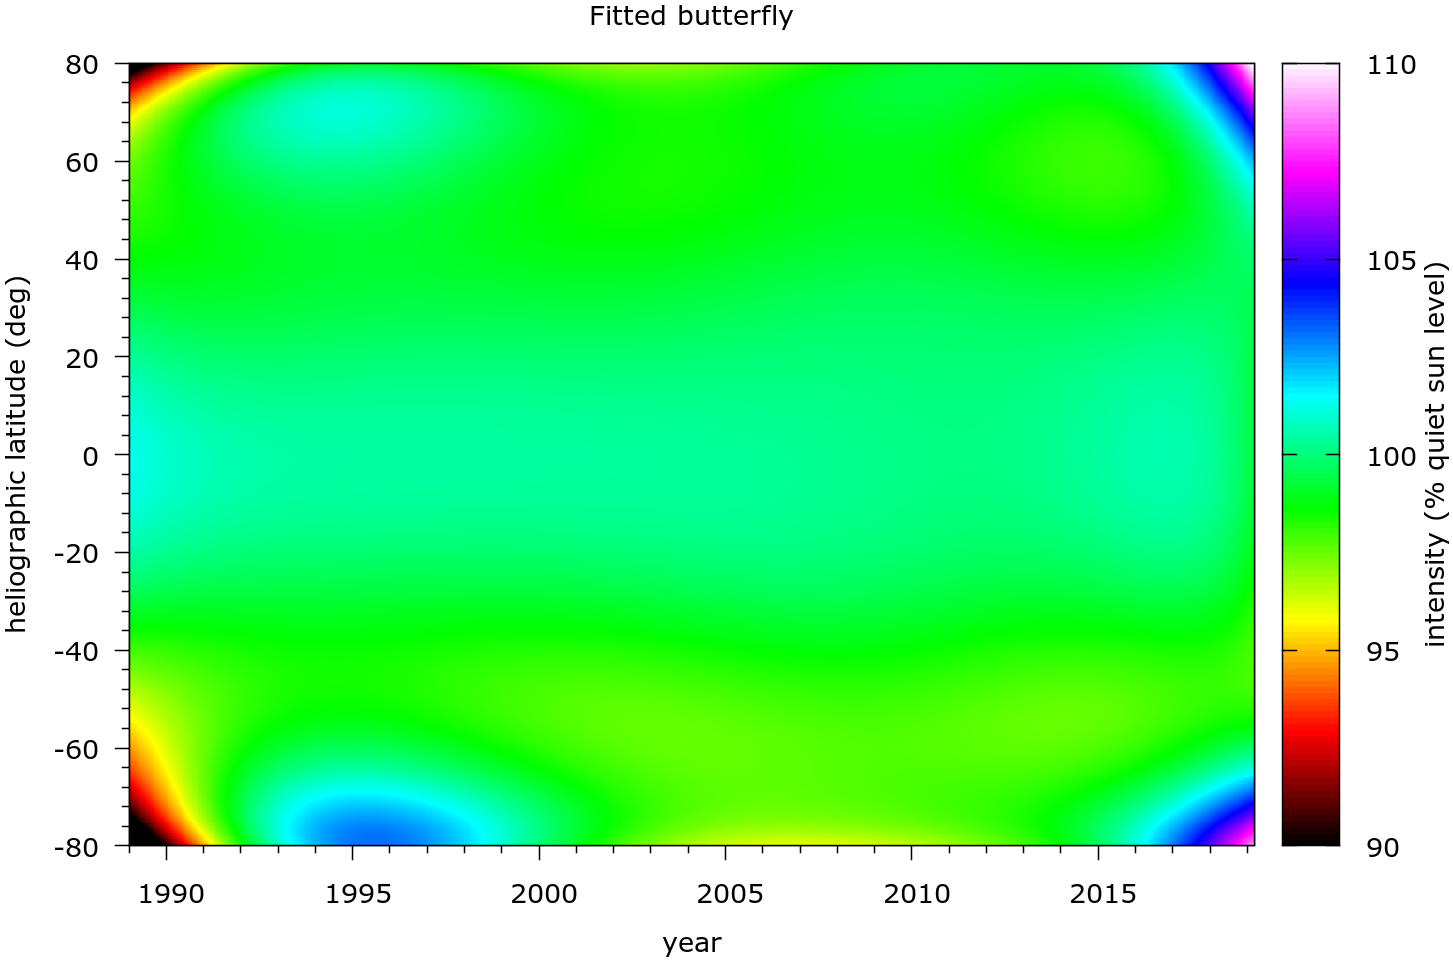
\includegraphics[width=8.5cm]{limbmodel_butterfly1.png}
%\caption{Idealized butterfly diagram showing cyclic behaviour at high %latitudes.}
%\label{limb_butterfly1}
%\end{figure}


%\subsection{Limb correction model}
%\begin{figure}
%\centering
%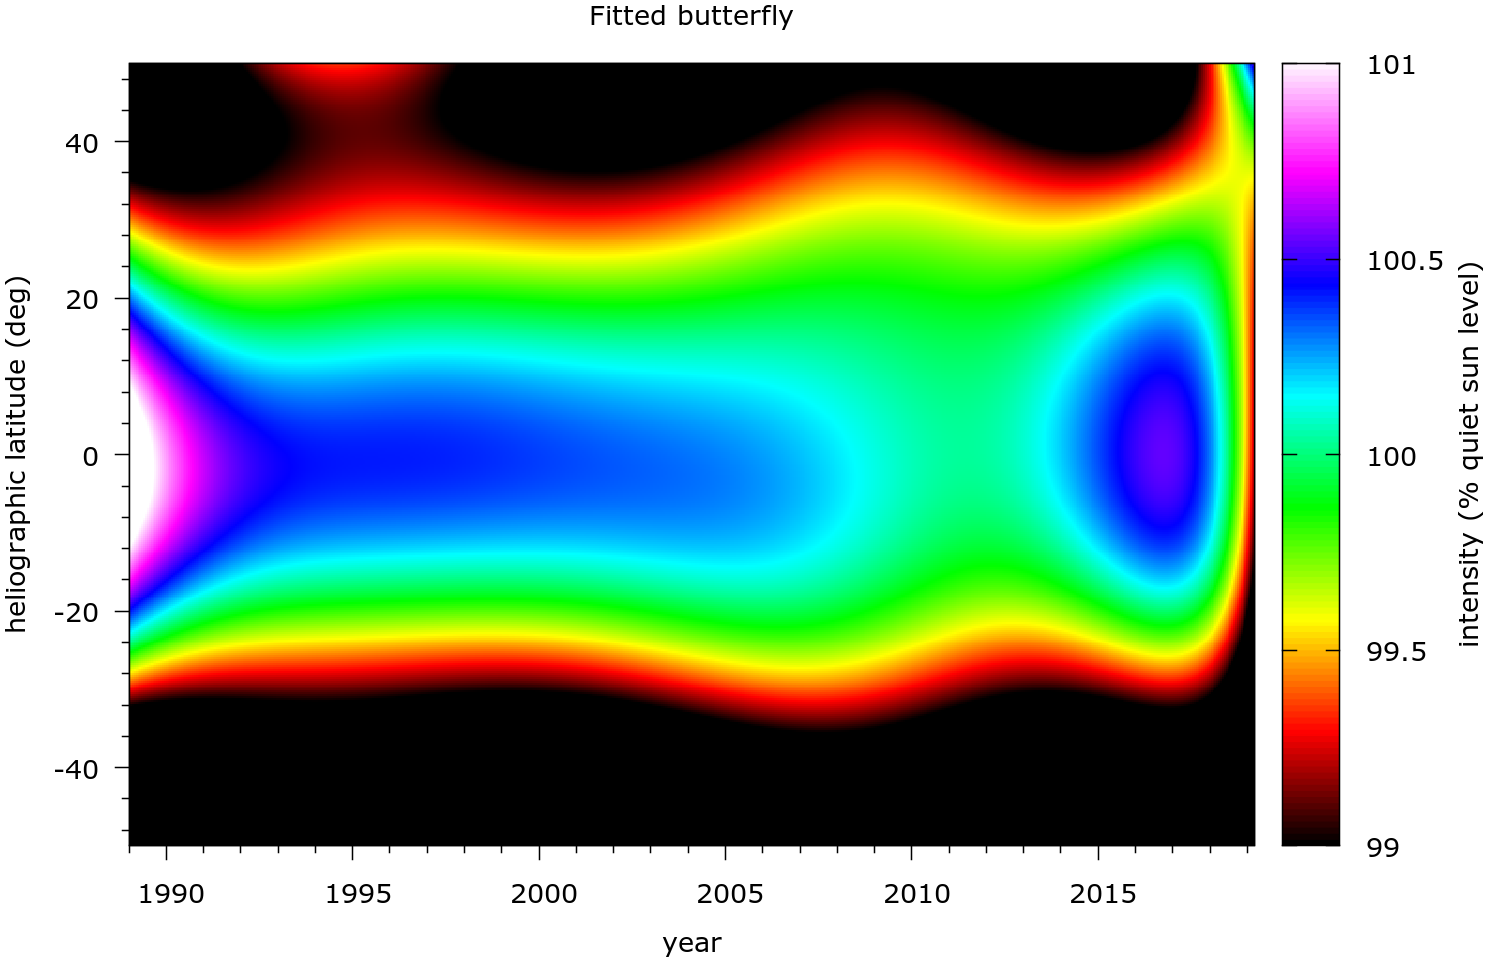
\includegraphics[width=8.5cm]{limbmodel_butterfly2.png}
%\caption{Idealized butterfly diagram with emphasis on the low %latitudes.}
%\label{limb_butterfly2}
%\end{figure}


%-------------------------------------- Two column figure (place early!)




%------------------------------------------------------------------------------
\section{Results}\label{sect:results}
\fag{To do: identify other observations/publications on polar magnetic cycles to compare with
Fig.~\ref{butterfly_clear_corr}. MJK: The Srivastava et al., 2018 paper should give plenty of refences. And perhaps more references can be found from those papers. Check Potsdam publications.}\\

%FAG added
From the series of specimen maps as processed using methods in 
Section\,\ref{sect:methods}, but without applying the limb correction model
(Section\,\ref{sect:limb}), we construct the radio butterfly diagram  
displayed in Fig.\,\ref{butterfly_clear_raw}

%------------------------------------------------------------------------------
\begin{figure}
\centering
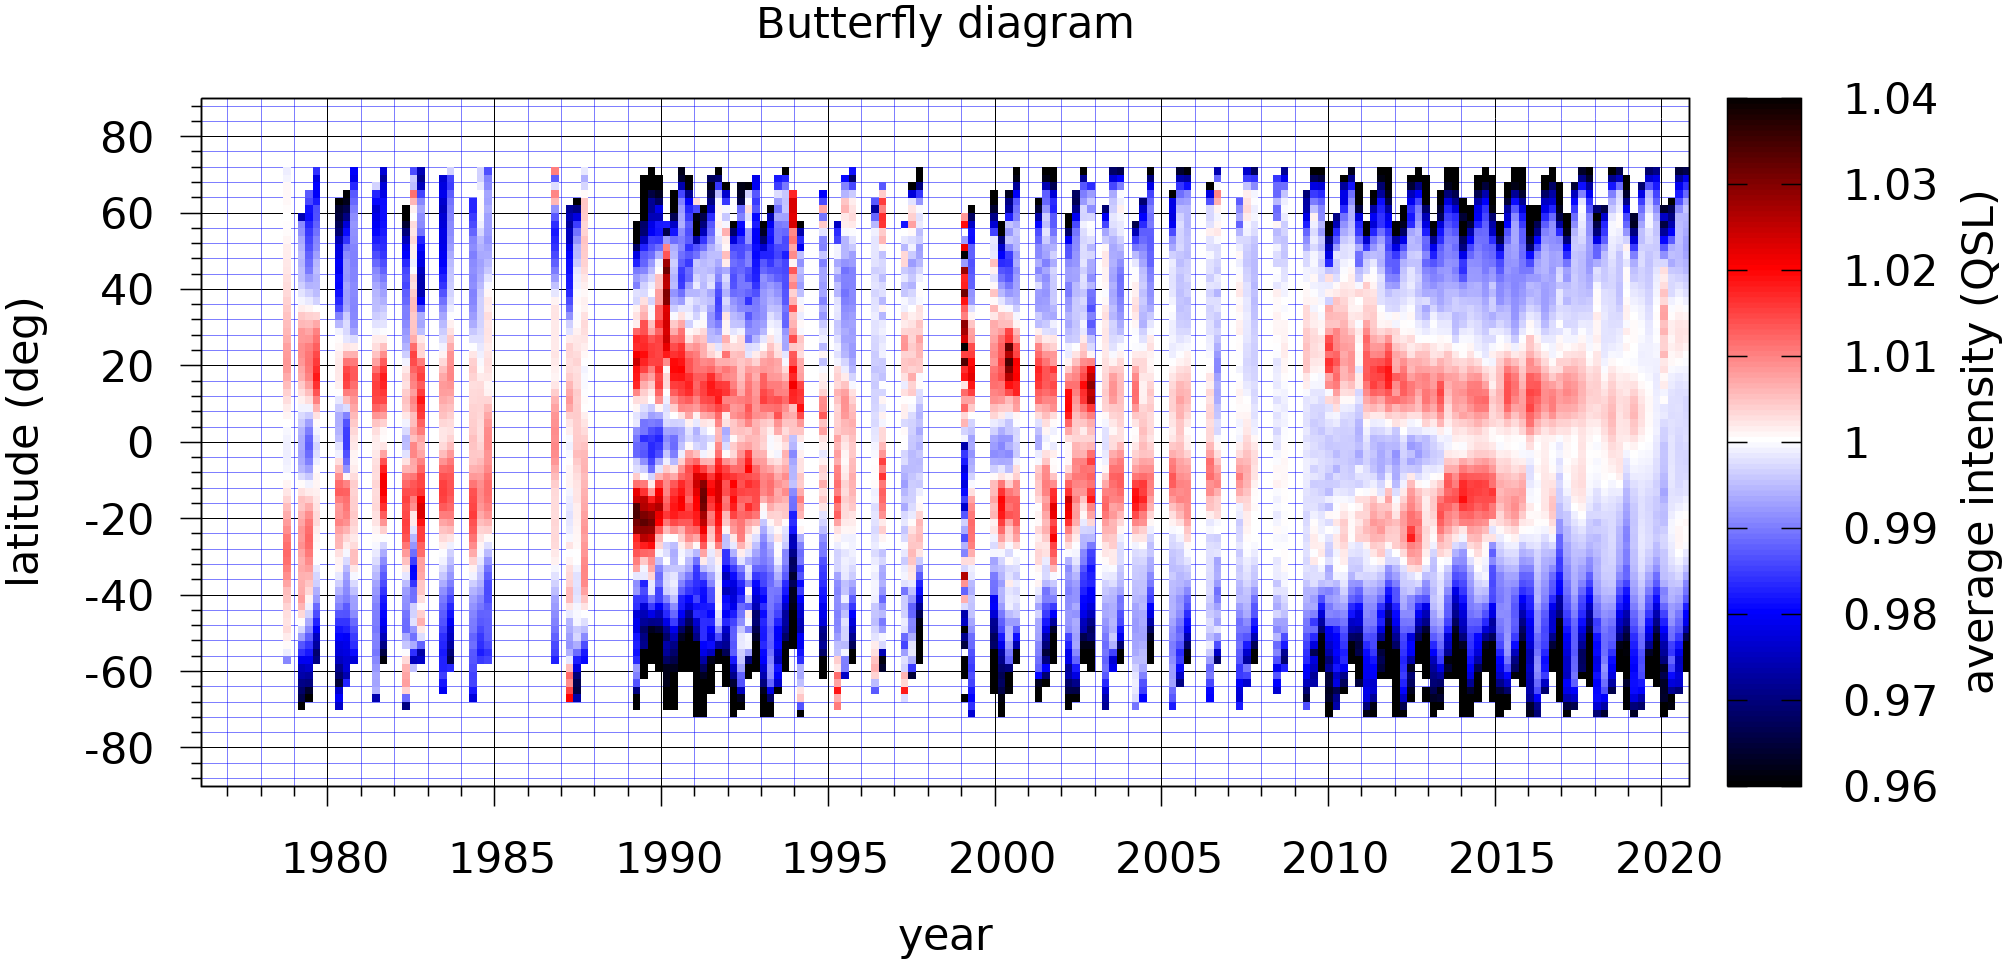
\includegraphics[width=8.5cm]{butterfly_clear_raw.png}
\caption{Solar intensity at all heliographic latitudes on $\si{37}{GHz}$ over cycles 21 to 24. Averaged over samples for which $r_i \le 0.9$ to avoid beam mixing with the background.
}
\label{butterfly_clear_raw}
\end{figure}
%------------------------------------------------------------------------------
%FAG. i think this has now been done
%\fag{(later) obtain same period of photospheric sunspot numbers
%Tabulate the timespans and line fits for all eight.}\\

%FAG moved from above
Each specimen map has weight $w_i$, which is set as to balance the target set. 
There are more 
observations starting from year $2015$, while only a few maps for year $1989$. 
%MJK Often we do just the opposite: if there are less data for a certain epoch, then the weigth is lower because of that time interval in more uncertain. Please expand on the logic here.
Thus we will put more weight on the old 
maps. Summer days typically have dozens of maps as the observational day is long, while on winter there are only a few maps per day.

We get more samples from the low heliographic latitudes, since a greater length of the solar equator is visible, 
compared to high latitude arcs. During summer, the solar north pole is visible to Earth, while we also get observations 
from high altitudes. During winter, we only observe the Sun at low altitude, and the solar south pole is visible. 
Further investigations are needed to exclude any bias effects arising from the unbalanced target set. However, having 
separate polynomials $P_n$ and $Q_m$ should reduce these risks. 
%MJK Good idea, but sounds like a task not necessary to undertake now? If the referee asks us to verify this risk, then we should do it. But, I comment it out for now...
%I suggest testing the optimization code with simulated 
%data.
%------------------------------------------------------------------------------
\begin{figure}
\centering
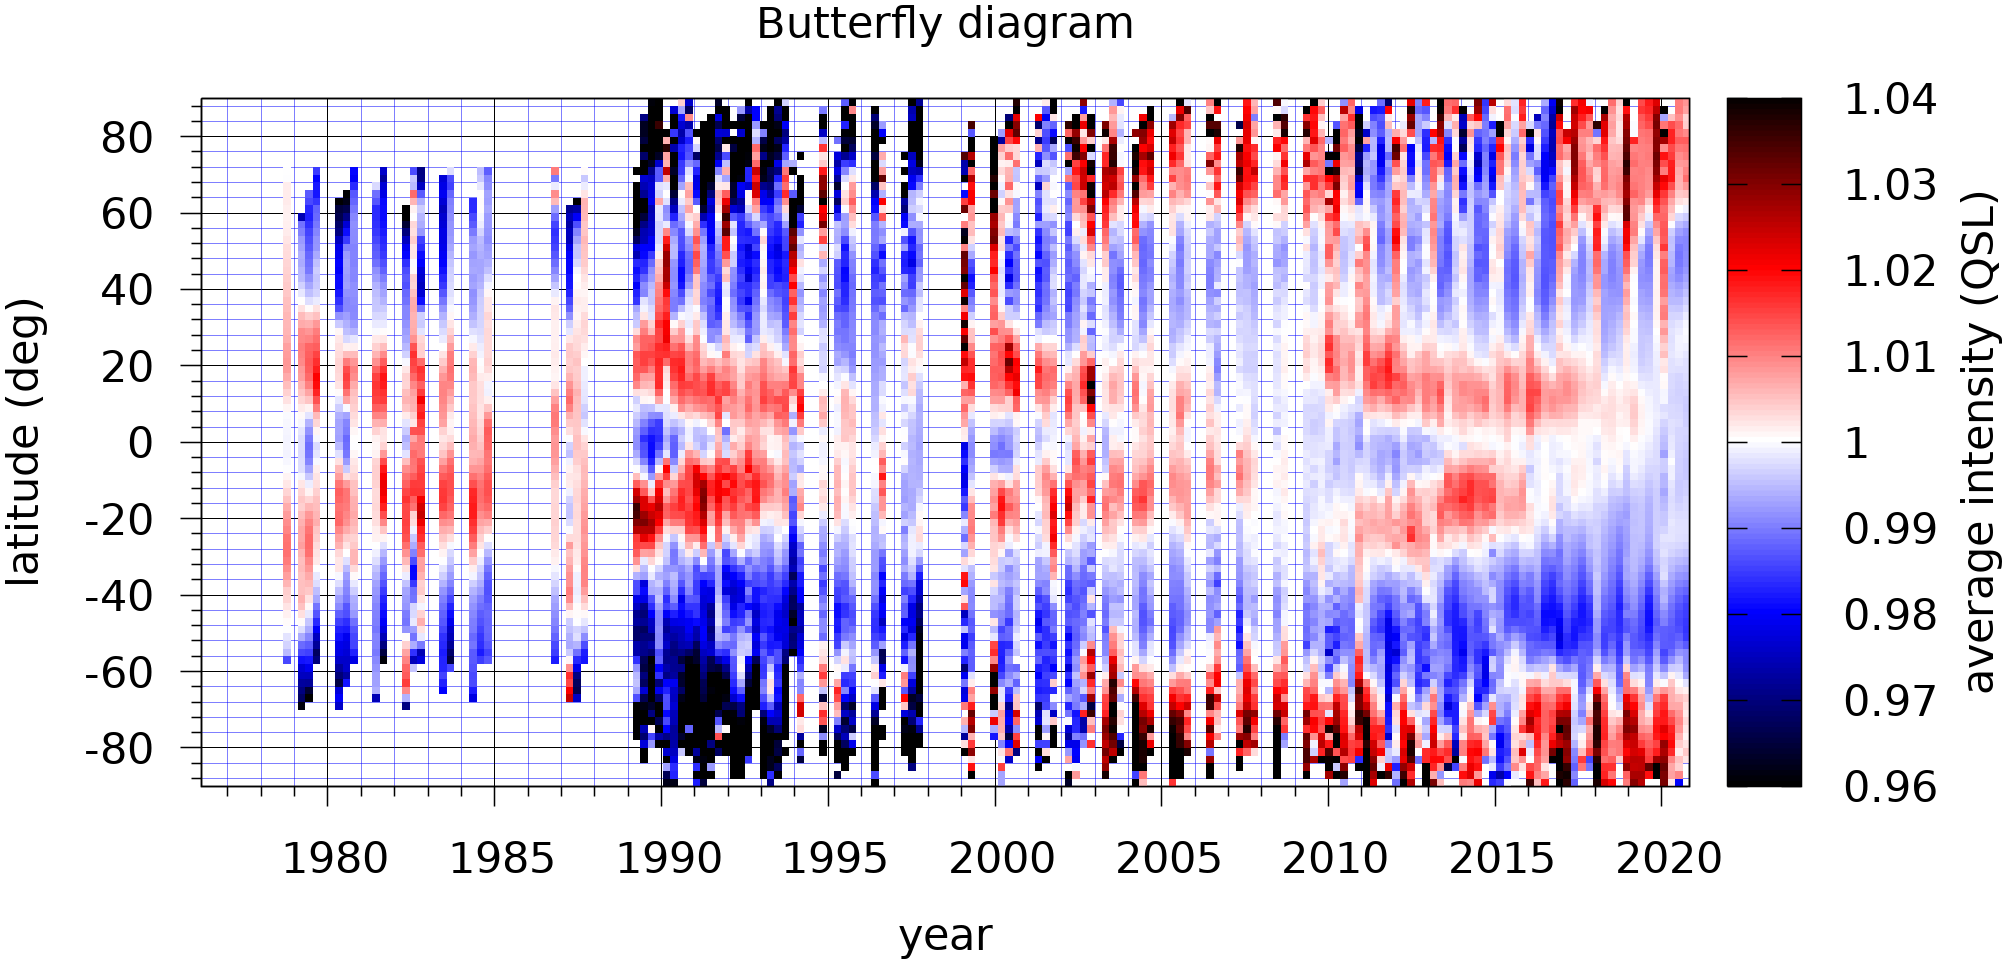
\includegraphics[width=8.5cm]{butterfly_clear_limb.png}
\caption{Solar intensity at all heliographic latitudes on $\si{37}{GHz}$ over cycles 21 to 24. Averaged over samples for which $r_i \le 1.0$ so that each sample intensity is corrected for beam mixing and limb brightening. This increases the available latitude range, bringing the polar magnetic cycle clearly visible.}
\label{butterfly_clear_corr}
\end{figure}
%------------------------------------------------------------------------------

%MJK The active region tracking tool is not yet described here. You are still planning to include that, right?
%------------------------------------------------------------------------------
\begin{figure}
\centering
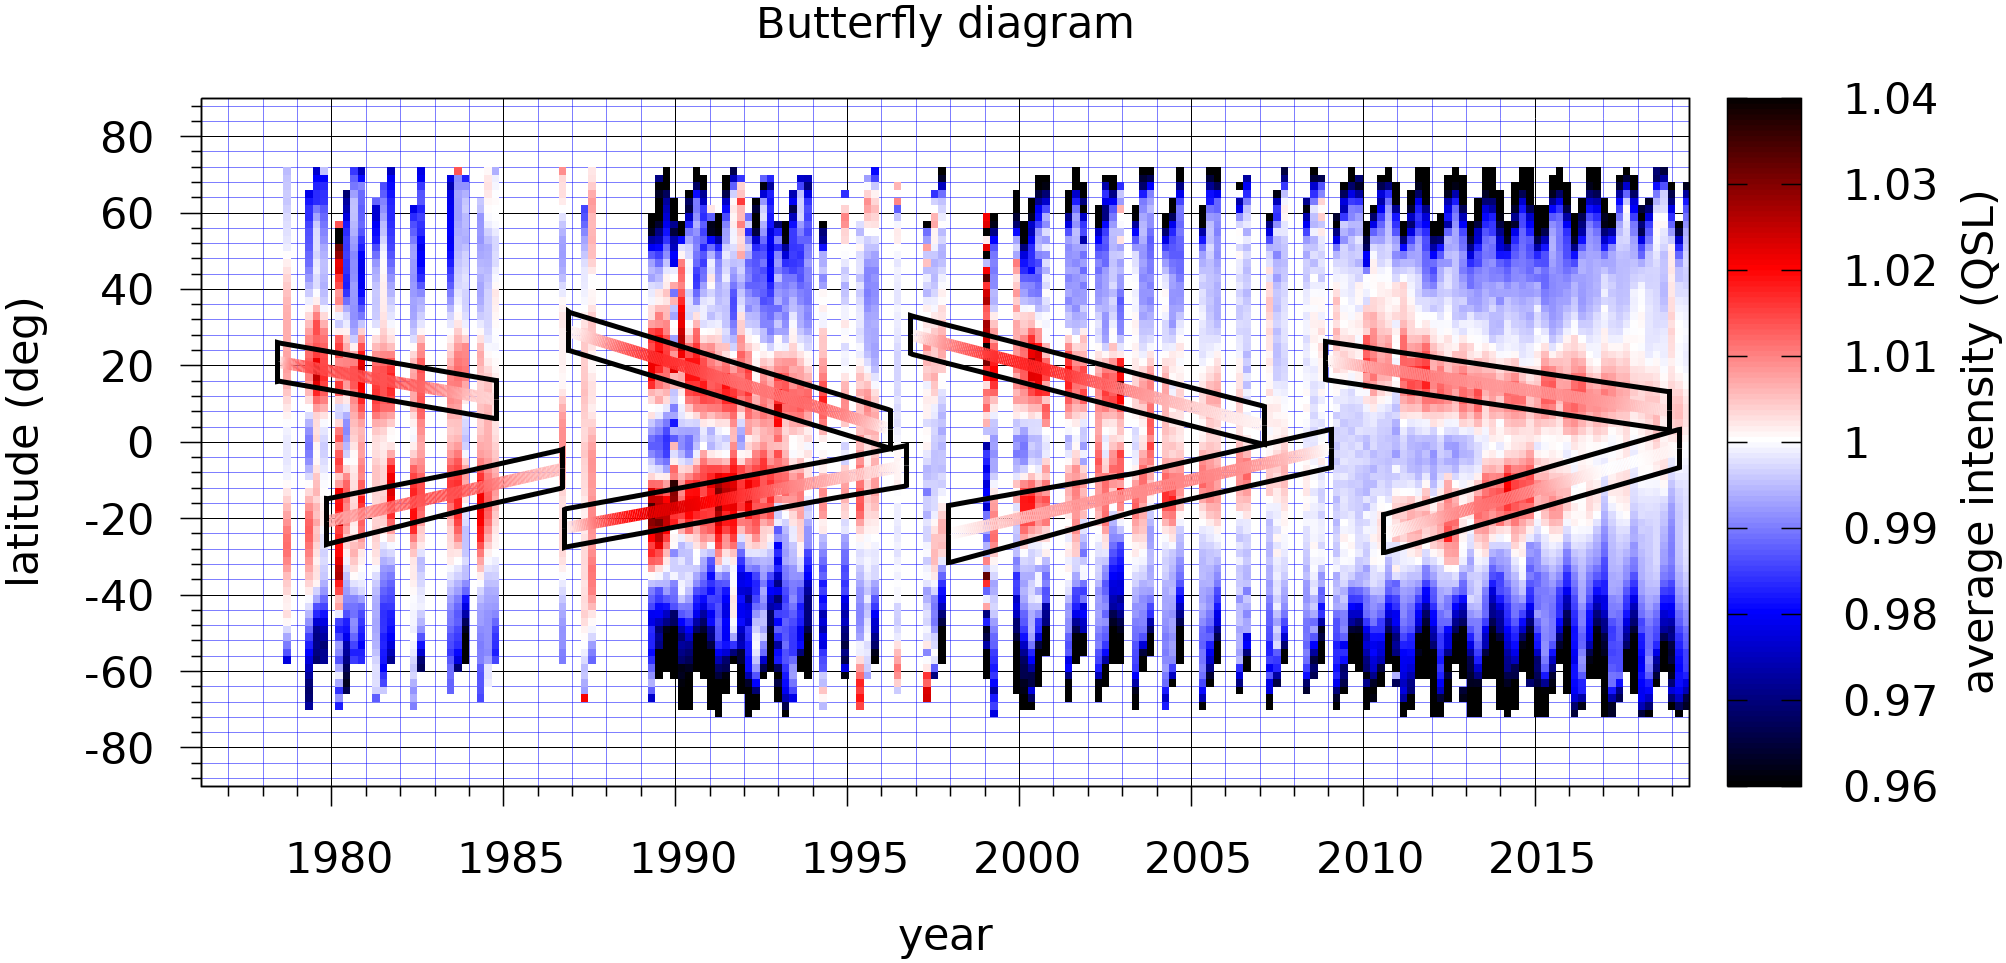
\includegraphics[width=8.5cm]{butterfly_wingfit_raw.png}
\caption{Butterfly wing patterns automatically fitted on top of Mets\"ahovi $\SI{37}{GHz}$ data (cf. Fig.~\ref{butterfly_clear_corr}).} 
\label{butterfly_wingfit_raw}
\end{figure}
%------------------------------------------------------------------------------

%------------------------------------------------------------------------------
\begin{figure}
\centering
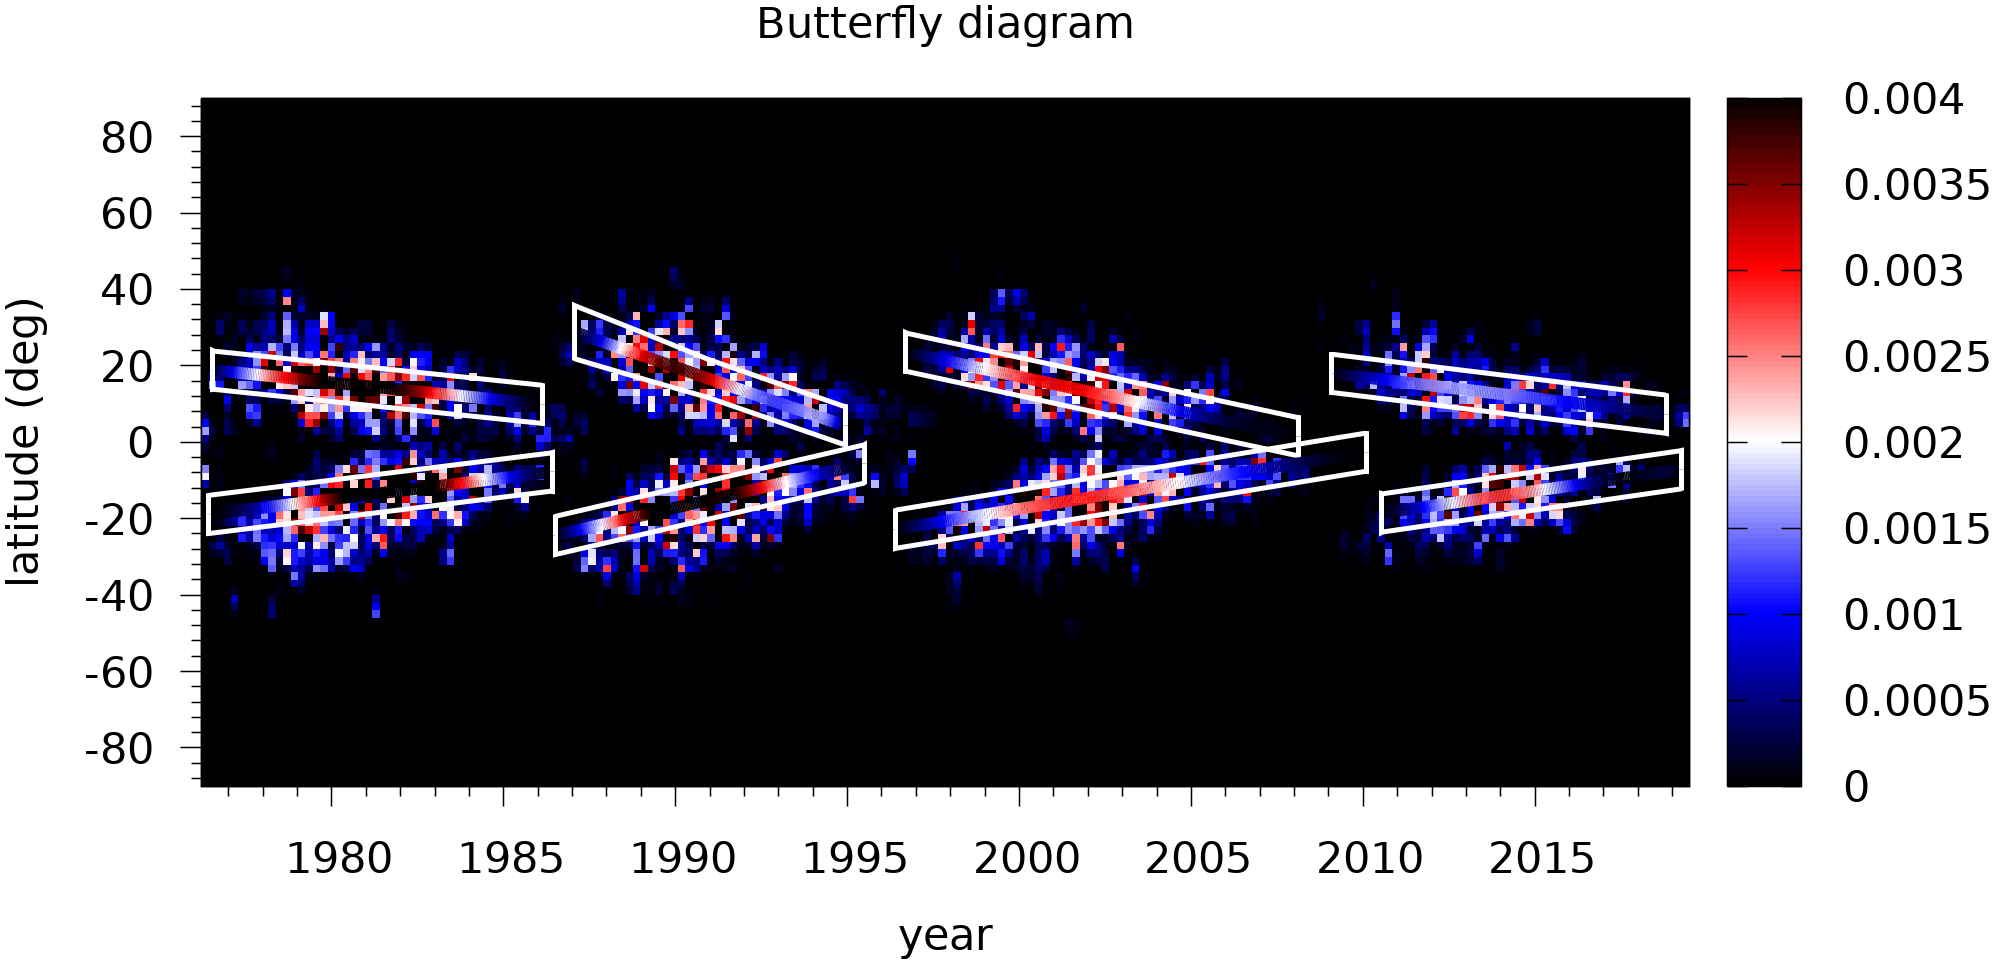
\includegraphics[width=8.5cm]{butterfly_wingfit_sunspot.png}
%FAG replace citation with url
%\caption{Butterfly wing patterns automatically fitted on sunspot data \cite{SUNSPOTDATA:1}. The sunspot cycle coincides with the radio cycle seen in Fig.. \ref{butterfly_wingfit_raw}. Comment: fix 21st cycle fitting.}
\caption{Butterfly wing patterns automatically fitted on sunspot data, for
cycles coinciding with the radio cycles in Fig.\,\ref{butterfly_wingfit_raw}.
Sunspot data courtesy Hathaway \& Upton, Solar Cycle Science,
Discover the Sun}
%\href{http://solarcyclescience.com/AR_Database/bflydata.txt}{http://solarcyclescience.com/AR_Database/bflydata.txt}.
\label{butterfly_wingfit_sunspot}
\end{figure}
%------------------------------------------------------------------------------

%------------------------------------------------------------------------------
\begin{table}
\caption{\label{tab:cycles}
Heliographic solar intensity butterfly fits for cycles 21 -- 24, by hemisphere.
Latitude Lat$_0$ and time $t_0$ at the start of each cycle, the slope of transition
towards the Equator, the time $t_{\rm end}$ at which each cycle is considered to have
ceased and the length of each cycle $\tau_{\rm cycle}$.
}
\begin{tabular}{l|ccccr}
\hline\hline
Cycle & Lat ($t_0$) & $t_0$ & slope                   & $t_{\rm end}$   & $	\tau_{\rm cycle}$ \\
      & [$\deg$]      &  [yr] & [$\deg{\rm yr}^{-1}$]   & [yr]            & [yr]                \\
\hline \\
21N & $+18.5^{\circ}$ & $1977.8$ & $-0.6$ & $1987.1$ &  9.3 \\
21S & $-19.1^{\circ}$ & $1979.3$ & $+1.8$ & $1986.8$ &  7.5 \\
\\
22N & $+31.0^{\circ}$ & $1987.1$ & $-3.0$ & $1996.7$ &  9.6 \\
22S & $-22.8^{\circ}$ & $1984.9$ & $+1.3$ & $1996.0$ & 11.1 \\
\\
23N & $+28.5^{\circ}$ & $1996.6$ & $-2.2$ & $2005.9$ &  9.3 \\
23S & $-25.4^{\circ}$ & $1998.2$ & $+2.4$ & $2008.4$ & 10.2 \\
\\
24N & $+21.6^{\circ}$ & $2008.2$ & $-1.2$ & $2019.5$ & 11.3 \\
24S & $-23.8^{\circ}$ & $2010.2$ & $+2.3$ & $2017.4$ &  7.1 \\
\\

\hline
\end{tabular}
\end{table}
%------------------------------------------------------------------------------

%------------------------------------------------------------------------------
\begin{table}
\caption{\label{tab:cycles_sunspot}
Sunspot data fits for cycles 21 -- 24, by hemisphere.
Latitude Lat$_0$ and time $t_0$ at the start of each cycle, the slope of transition
towards the Equator, the time $t_{\rm end}$ at which each cycle is considered to have
ceased and the length of each cycle $\tau_{\rm cycle}$.
}
\begin{tabular}{l|ccccr}
\hline\hline
Cycle & Lat ($t_0$) & $t_0$ & slope                   & $t_{\rm end}$   & $	\tau_{\rm cycle}$ \\
      & [$\deg$]      &  [yr] & [$\deg{\rm yr}^{-1}$]   & [yr]            & [yr]                \\
\hline \\
21N & $+17.5^{\circ}$ & $1977.6$ & $-0.8$ & $1985.6$ &  8.0 \\
21S & $-14.6^{\circ}$ & $1978.1$ & $+0.6$ & $1986.3$ &  8.3 \\
\\
22N & $+32.6^{\circ}$ & $1986.8$ & $-3.9$ & $1994.3$ &  7.5 \\
22S & $-24.1^{\circ}$ & $1986.4$ & $+2.1$ & $1994.8$ &  8.4 \\
\\
23N & $+24.3^{\circ}$ & $1996.5$ & $-1.9$ & $2006.3$ &  9.8 \\
23S & $-23.6^{\circ}$ & $1995.9$ & $+1.5$ & $2008.6$ & 12.7 \\
\\
24N & $+17.8^{\circ}$ & $2008.7$ & $-1.0$ & $2018.5$ &  9.8 \\
24S & $-18.9^{\circ}$ & $2010.3$ & $+1.4$ & $2017.8$ &  7.5 \\
\\

\hline
\end{tabular}
\end{table}
%------------------------------------------------------------------------------

%------------------------------------------------------------------------------
\begin{figure*}
\centering
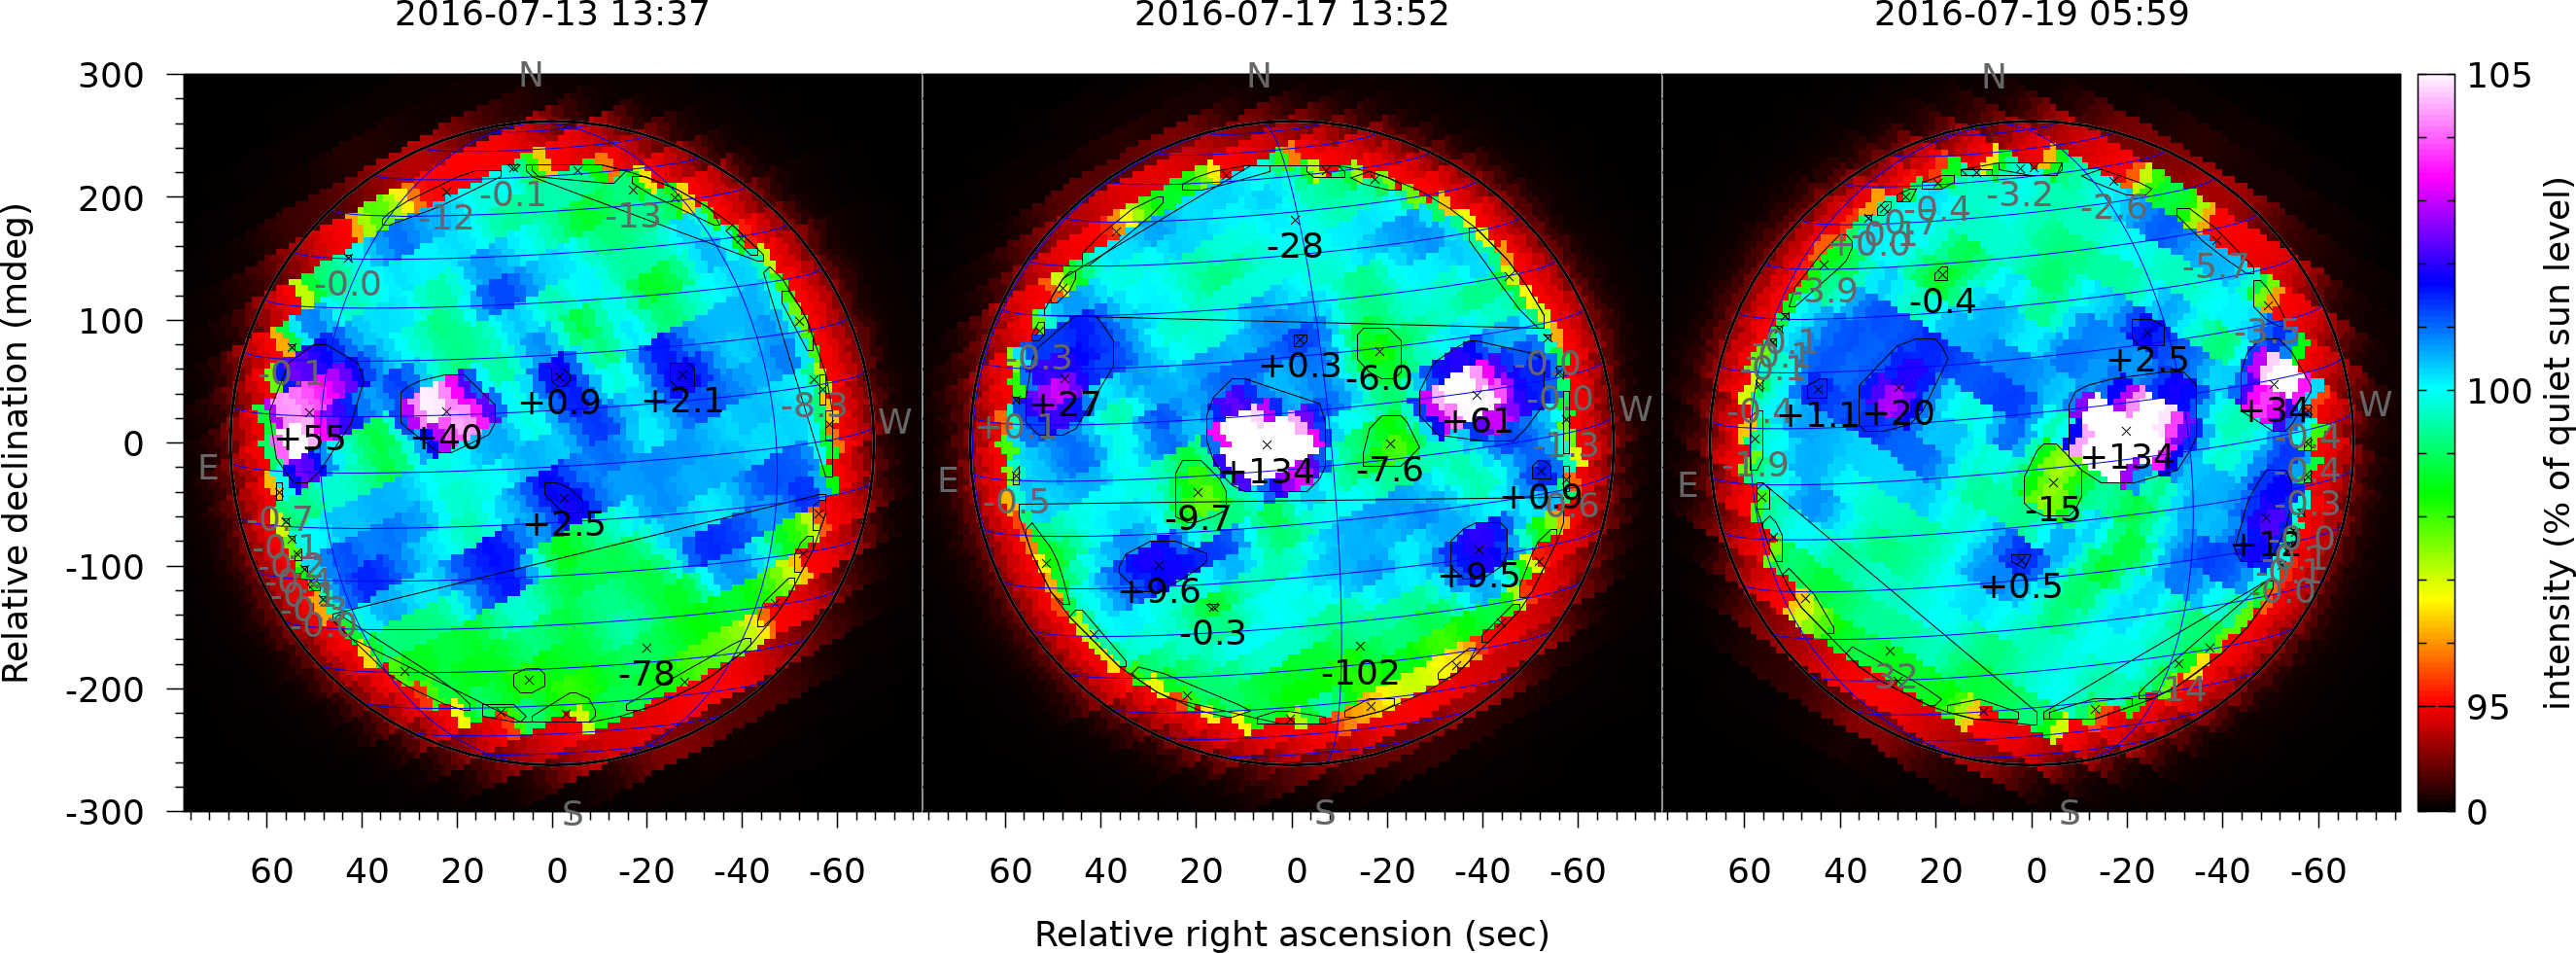
\includegraphics[width=\textwidth]{maptrack1.png}
\caption{Two active regions passing the visible disk as the Sun rotates.}
\label{maptrack1}
\end{figure*}
%------------------------------------------------------------------------------

%------------------------------------------------------------------------------
\begin{figure} \centering 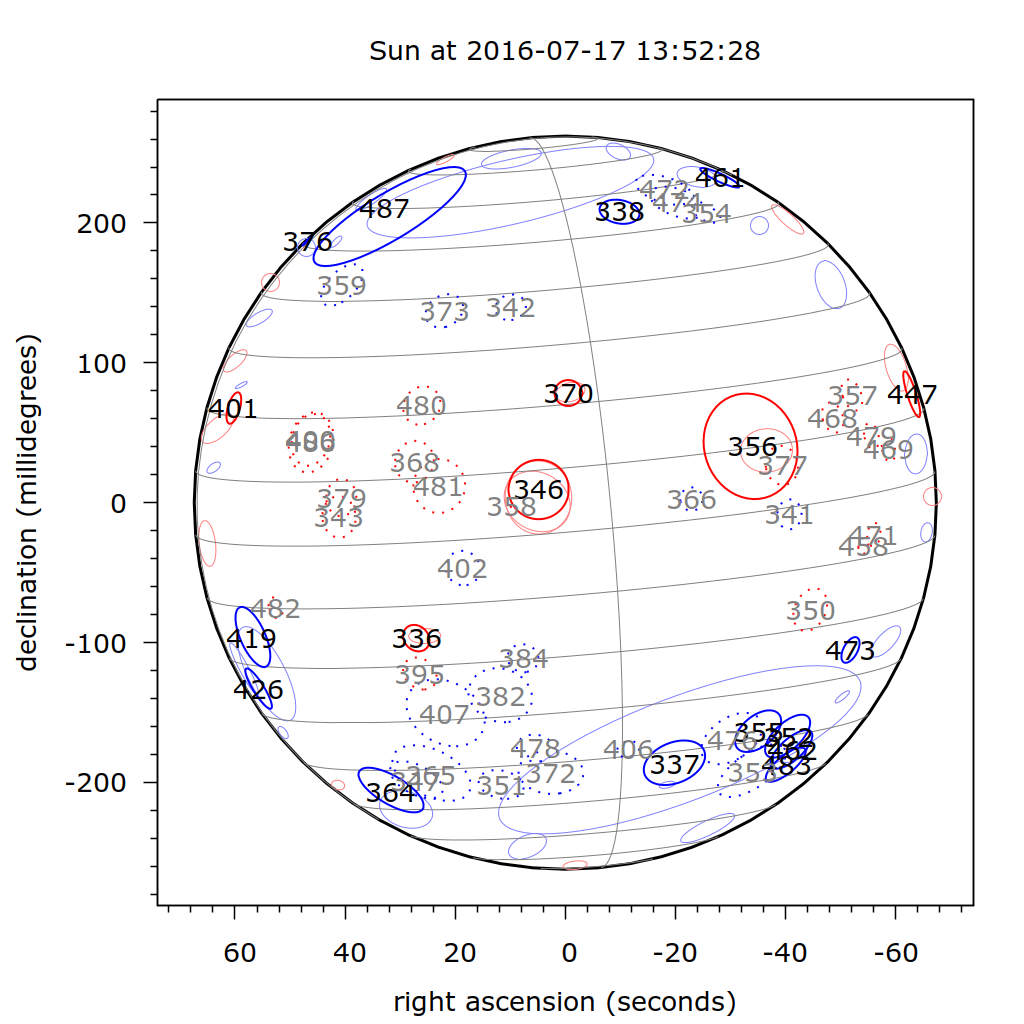
\includegraphics[width=8.8cm]{maptrack2.png} \caption{Tracked regions are shown with red 
ellipses for bright regions and with blue ellipses for dim regions. Based on earlier and later sunmaps, we can often 
expect a weak region to be visible at known heliographic coordinates. When the region nevertheless is found on this map, 
we show it with a dashed ellipse. The active regions 346 and 356 are clearly visible in Fig.~\ref{maptrack1}.} 
\label{maptrack2} \end{figure}
%------------------------------------------------------------------------------

%------------------------------------------------------------------------------
\section{Discussion}\label{sect:discussion}

We have featured a software package for processing solar maps. The radio observations reproduce the butterfly diagram 
observed on sunspot data, and are able to see the extended cycle at high latitudes. We automatically detect bright and 
dim features from the maps and track them from map to map. This allows us to analyze their migration on heliographic 
surface. We also obtain various structural information from these regions.

  \subsection{Determining radius by limb intensity} \label{sect:radius_method1}

  The first method is performed using the all MRO solar maps of the cycle $24$, combining c.a. $75800$ maps. For each 
  map, we perform the calibration procedure described in Section~\ref{sect:source} and concatenate the samples into a 
  big list of c.a. $2 \times 10^8$ samples. The next step in the analysis involves five data fields per sample:
  \begin{itemize}
  \item Time (on solar cycle 24): $t_j$.
  \item Heliographic latitude: $l_j$.
  \item Distance from the center of disk, relative to the apparent radius of the disk: $r_j$.
  \item Altitude of observation, angle with respect to horizon at MRO: $a_j$.
  \item Normalised intensity: $v_j$.
  \end{itemize}

  Here the index $j$ is mapped to some sample $s_i$ on some map $S$, and $j$ runs over all the maps of cycle $24$. The 
  distance $r_j$ is zero at the center and unity at the boundary of the disk.
    The polynomial $A$ should compensate for the butterfly diagram of cycle $24$, which is intensity vs. time and heliographic latitude. Meanwhile, the polynomial $B$ should compensate any limb effects.
  We emphasize the boundary at $r=1$ by transforming to $\rho$ as:
  \eqnl{physical_radius_trans}{
  \rho_j := \arctan \left( \kappa \left( r_j - 1 \right)\right) \; \text{with} \; \kappa = 8.8 \text{.}
  }
  We then perform an optimization to 
  minimize a target function:
  \eqnl{physical_radius_target}{
  U(\bm{x}) = \sum \limits_{j=1}^{N} \left( A(\bm{x},t_j,l_j) B(\bm{x},\rho_j,a_j) - v_j \right)^2 \text{.}
  }
  Here the functions $A$ and $B$ are two-dimensional polynomials of $(t,l)$ and $(\rho,a)$, respectively, with coefficients obtained from individual elements of the vector $\bm{x}$. We write the polynomials as:
  \eqnl{physical_radius_polynomials}{
  A(\bm{x},t,l) = \sum \limits_{g=0}^{4} \sum \limits_{h=0}^{4-g} c_{g,h} t^g l^h \; \text{and} \;
  B(\bm{x},\rho,a) = \sum \limits_{g=0}^{6} \sum \limits_{h=0}^{6-g} d_{g,h} \rho^g a^h \text{.}
  }
  The vector $\bm{x}$ is constructed from coefficients $c_{g,h}$ and $d_{g,h}$. With current selection of degrees $4$ 
  and $6$ for polynomials $A$ and $B$, respectively, we will have $6*5/2 + 8*7/2 = 43$ elements in $\bm{x}$. The element 
  $\bm{x}^{(0)}$ refers to $c_{0,0}$, and $\bm{x}^{(15)}$ refers to $d_{0,0}$.

  The optimization is performed iteratively. We start with an initial vector $\bm{x}_0$, where each element 
  $\bm{x}_0^{(g)}$ will be a small random value, except for $g=0,15$where we start with $\bm{x}^{(g)} = 1$, thus 
  setting $c_{0,0} = d_{0,0} = 1$ and giving a flat solar cycle and flat disk with some noise. We proceed with iterative 
  steps of quadratic optimization. At each step $m$ we calculate the gradient $\bm{g}_m := \nabla U(\bm{x}_m)$ and the Hessian of $U(\bm{x_m}$, which should be $H_m$. Basically we search for the point of zero gradient iteratively, starting from $m=0$:
  \eqnl{physical_radius_step}{
  \bm{x}_{m+1} := \bm{x}_m - H_m^{-1} \bm{g}_m \text{.}
  }

  However, this naive approach will easily run into trouble when we are far from the actual minimum of $U(\bm{x})$. For 
  this reason, we have a developed a more rebust scheme which first diagonalizes $H_m$. The algorithm tries to choose 
  how much to advance along each eigenvector of $H_m$. The algorithm tries to avoid the eigenvectors accociated with 
  negative eigenvalues, but will eventually descend away from possible saddle points.
  
  We force the disk to be flat at the center, thus $\frac{\partial B}{\partial r}\big|_{r=0} = 0$. This limits the 
  subspace allowed for $\bm{x}$ and reduces the amount of degrees of freedom in the setting to $37$. The optimization stops successfully (converges) at step $m$ when we observe that:
  \begin{itemize}
  \item $H_m$ is positively definite in the allowed subspace.
  \item The next step $\bm{x}_{m+1} - \bm{x}_{m}$is comparable to numerical precision.
  \item $U(\bm{x}_{m+1})$ is equal or slightly greater than $U(\bm{x}_m)$ due to limits in the numerical precision.
  \end{itemize}

  Having optimized $U(\bm{x}_{m})$ at sufficient amount of steps ($m$), we define the limb profile $L(r)$ for a given altitude $a = 30^{\circ}$ as:
  \eqnl{physical_radius_limb}{
  L(r) := \frac{B(\bm{x}_m, \rho(r), a)}{B(\bm{x}_m, \rho(1/3), 30^{\circ})} \text{.}
  }
  We thus state that the reference Sun is observed on altitude $30^{\circ}$ above horizon. The function $L(r)$ is a $6$:th degree polynomial of $\rho(r)$. We search for the value $\s{r}{limb}$ where:
  \eqnl{physical_radius_limb2}{
  L(\s{r}{limb}) = 0.5 \text{.}
  }
  We start the above process using a reasonable value for the physical radius of the Sun, namely, $R_{\astrosun}^{(0)}$. 
  Starting from $q=0$, the process gives a value of $\s{r}{limb}^{(q)} \approx 1$. When there is a slight deviation from 
  unity, we correct that into the physical Sun radius by setting:
  \eqnl{physical_radius_iteration}{
  R_{\astrosun}^{(q+1)} := Q_{\astrosun}^{(q)} * \s{r}{limb}^{(q)}
  }
  After a few steps, the radius $R_{\astrosun}^{(q+1)}$no longer evolves. So far we have obtained a convergent value of $R_{\astrosun}^{(\infty)} \approx 7.176 \times 10^8 \mathrm{m}$.

  \subsection{Determining radius by inversion model} \label{sect:radius_method2}

  We start with a predefined $R_{\astrosun}$ and sweep the reasonable interval $[6.90, 7.25] \times 10^8 \mathrm{m}$. 
  Currently the model works on a few $n \approx 14$ maps at once. This does not analyze a full solar cycle but rather a 
  single day of observations. The model involves a centering scheme similar to that in described fully in 
  Section~\ref{sect:s_curve}, \ref{sect:initial-centering}, \ref{sect:further_optimization}, and~\ref{sect:outliers_limb}. However, this 
  scheme involves solving the inversion problem several times and constructing the limb model for each map individually 
  each time the inversion problem is solved. This approach tackles not only the different altitude of observation 
  depending on time of day, but also varying weather and atmospheric conditions which affect the telescope beam. The 
  model omits outlier samples using a similar recursive scheme as described completely in 
  Section~\ref{sect:outliers_limb} and~\ref{sect:outliers_disk}.

  Each sample constitutes of four values: $s_j = (t_j, x_j, y_j, v_j)$, where $t_j$ is time, $v_j$ is calibrated intensity, 
  and $(x_j,y_j)$ describe the position of the sample on the calibrated disk as right ascension and declination 
  relative to the center of the Sun. We parametrize the telescope beam $B(z^2)$with a polynomial times a gaussian function of known width $\sigma$:
  \eqnl{inversion_beam}{
  B(z^2) = e^{-\frac{z^2}{2 \sigma^2}} \sum \limits_{g=0}^{4} b_g z^{2g} \text{.}
  }
  Here $z$ refers to the relative angle between a source element and the observed sample. We only need even powers of $z$ in the polynomial factor since the beam is radially symmetric. We produce an estimate $e_j$for each sample $s_j$ through integrating over the telescope beam:
  \eqnl{inversion_beam2}{
  e_j = \intef{x^{\prime}}{-\infty}{+\infty}{ \intef{y^{\prime}}{-\infty}{+\infty}{ f(x^{\prime}, y^{\prime}) B \left( \left( x - x^{\prime} \right)^2 + \left( y - y^{\prime} \right)^2 \right)}}
  }

  The integral in Equation~\ref{inversion_beam2} is evaluated numerically using Gaussian quadratures. There are 
  $7$cocentric rings of quadrature points around the sample $(x_j,y_j)$. The radii of the rings come from a quadrature 
  rule with gaussian weight function. Each ring contains $6$ quadrature points, and the placement of the points along the ring comes from a linear 
  quadrature rule. Various ad hoc solutions are implemented in order to handle singularities and discontinuities at the 
  disk boundary as well as to maintain sufficient numerical stability.

  Once the quadratures are implemented, we arrive into a linear summation formula for each sample $s_j$. The coefficients $\xi_{j,i}$ are calculated as a products of the corresponding ring and point quadrature coefficients.
  \eqnl{inversion_beam3}{
  \epsilon_j = \sum \limits_{i=1}^{42} \xi_{j,i} f(x^{\prime}_{j,i}, y^{\prime}_{j,i} \approx e_j \text{.}
  }

   We project each of the sky coordinates $((x^{\prime}_{j,i}, y^{\prime}_{j,i})$ at time $t_j$ on the spherical solar 
   surface with radius $R_{\astrosun}$. This gives us the heliographic latitude $l^{\prime}_{j,i}$ of the point where the line of sight is incident with the solar surface. We denote by $\alpha_{j,i}$ the angle of incidence.
   
  We have a polynomial $A$ for describing the current phase of the solar 
   cycle.
   
  
%------------------------------------------------------------------------------
\subsection{The big picture}

The radio samples in solar maps can be divided into three categories: \begin{itemize} \item Quiet Sun background \item 
Bright features \item Dim features. \end{itemize} Bright and dim features are a signal of activity. Our intention is to 
study the development and lifetime of this activity, for which we have developed algorithms for extracting these 
features from the maps. We also need to understand how the quiet Sun behaves, and for this purpose, any activity is 
excluded. The brightness of these quiet areas supposedly depend on heliographic latitude and the solar cycle. When these 
regions are observed, the ap:qparent brightness also depends on the distance from the visual center, due to atmospheric 
and antenna beam convolution effects. We want to measure these effects in order to properly compensate for them. We do 
not want any activity to affect these measurements, so we will benefit if we already know where the active and dim 
regions are. The compensation model consists of an implicit butterfly as well as a radial model for the brightness, and 
the expected brightness of a quiet region is taken as a product of these two.

Accurately understanding the radial effects in observations benefits the centering algorithm. Also, we benefit from 
prior knowledge of active regions since they can be excluded in the statistics which we feed into the centering 
algorithm. Otherwise the features at the limb would bias the center of the map.

Radial model also increases the dynamic radius of the map, and we are able to detect bright and dim features at the 
limb, although with increased noise. Each part of the model will benefit other parts and result in a data model of progressive accuracy, as outlined in Fig.~\ref{roadmap}.

Ultimately, all these three aspects, quiet, bright, and dim features, have a known physical origin, and their 
statistical appearance and characteristics can be reproduced in appropriate simulations.

%\begin{figure*} 
%\centering \scalebox{0.75}{\begin{tikzpicture}
%\node[textarea] (maps) {Mets\"ahovi solar intensity maps};
%\node[largeblock, right=5mm of maps] (calib) {\setlength\tabcolsep{0pt} \begin{tabular}{m{23mm}m{15mm}} Disk fitting and intensity calibration & 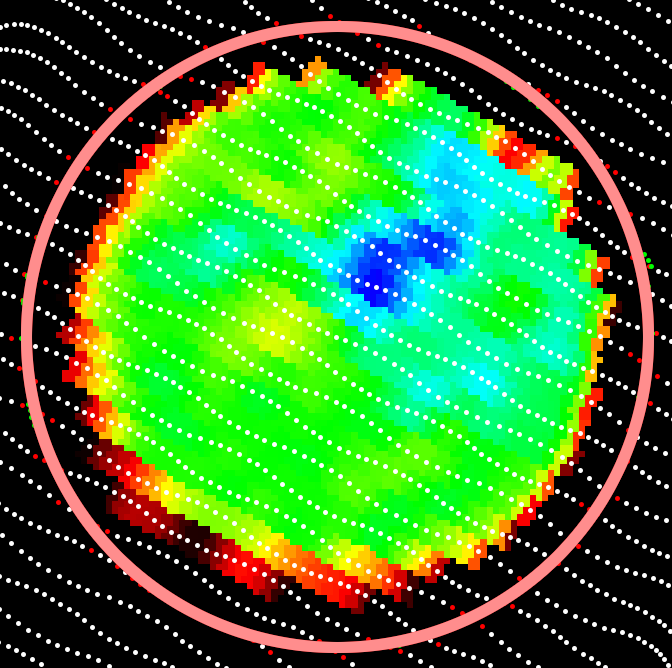
\includegraphics[width=15mm]{calib.png} \end{tabular}};
%\node[block, below right=15mm and -25mm of calib] (estimate) {Solar disk estimate from least squares approach};
%\node[largeblock2, above right=10mm and -50mm of calib] (dbase) {\setlength\tabcolsep{0pt} \begin{tabular}{m{23mm}m{25mm}} Bright and dim region database & 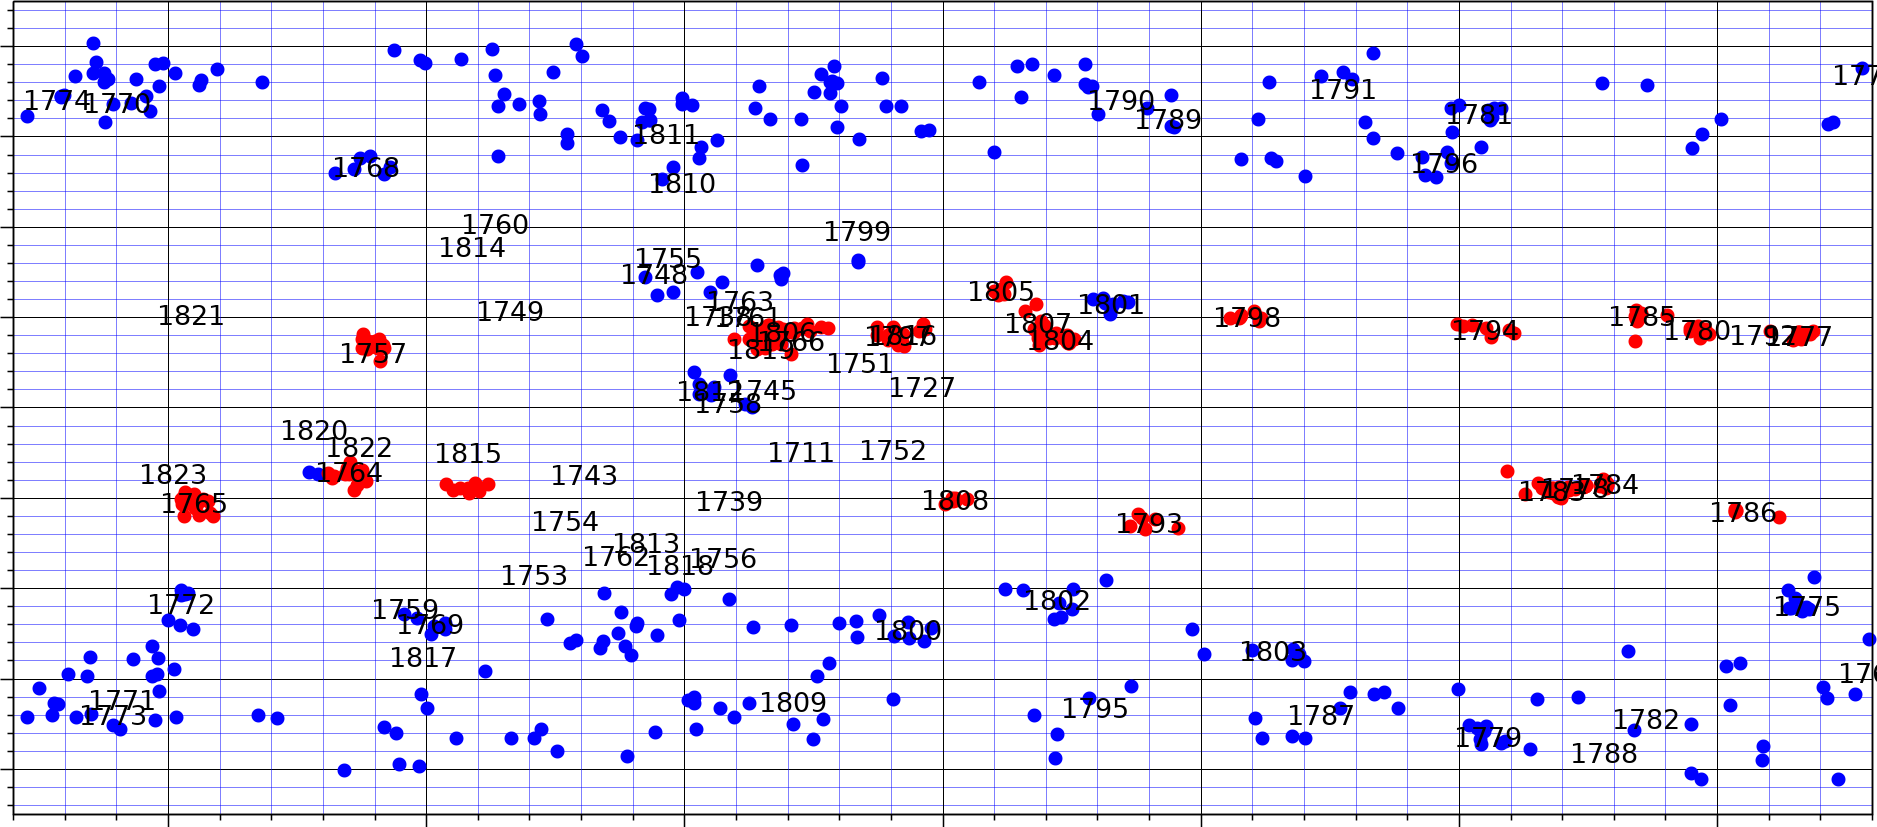
\includegraphics[width=25mm]{dbase.png} \end{tabular}};
%\node[largetextarea2, above right=-8mm and 5mm of estimate] (ibutterfly) {\setlength\tabcolsep{0pt} \begin{tabular}{m{23mm}m{25mm}} Implicit model for quiet sun butterfly & 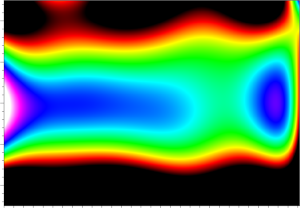
\includegraphics[width=25mm]{ibutterfly.png} \end{tabular}};
%\node[largetextarea2, below right=-8mm and 5mm of estimate] (lmodel) {\setlength\tabcolsep{0pt} \begin{tabular}{m{23mm}m{25mm}} Limb brightening and beam convolution model & 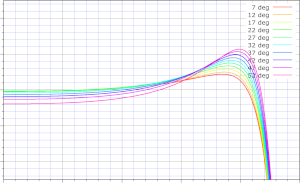
\includegraphics[width=25mm]{lmodel.png} \end{tabular}};
%\node[largetextarea, right=6mm of calib] (qbutterfly) {\setlength\tabcolsep{0pt} \begin{tabular}{m{23mm}m{25mm}} Quiet sun butterfly & 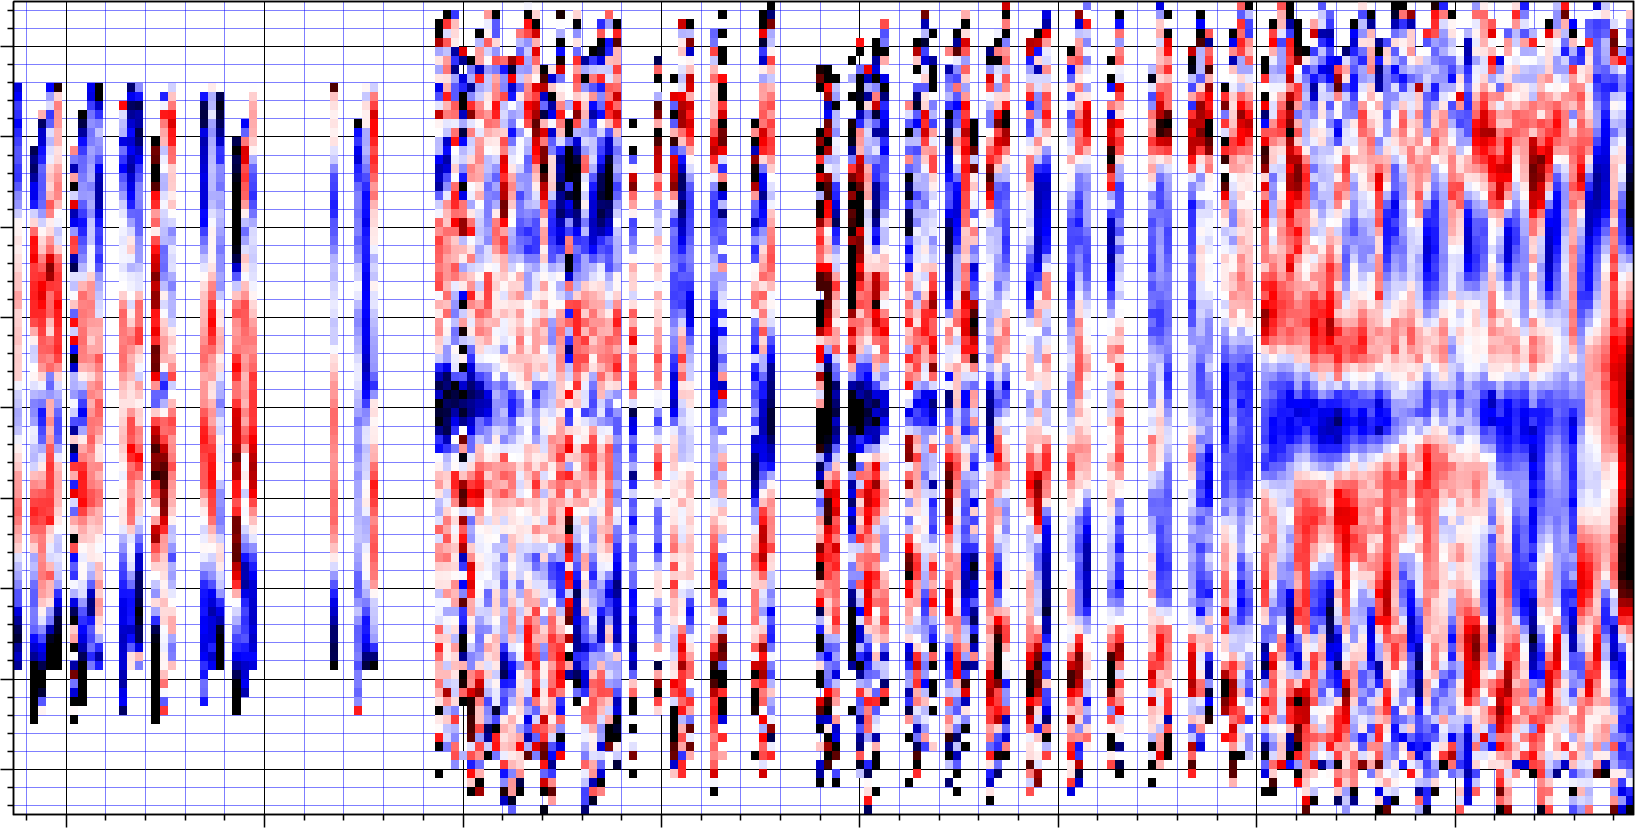
\includegraphics[width=25mm]{qbutterfly.png} \end{tabular}};
%\node[largetextarea, below right=-8mm and 5mm of dbase] (hbutterfly) {\setlength\tabcolsep{0pt} \begin{tabular}{m{23mm}m{25mm}} Bright region butterfly & 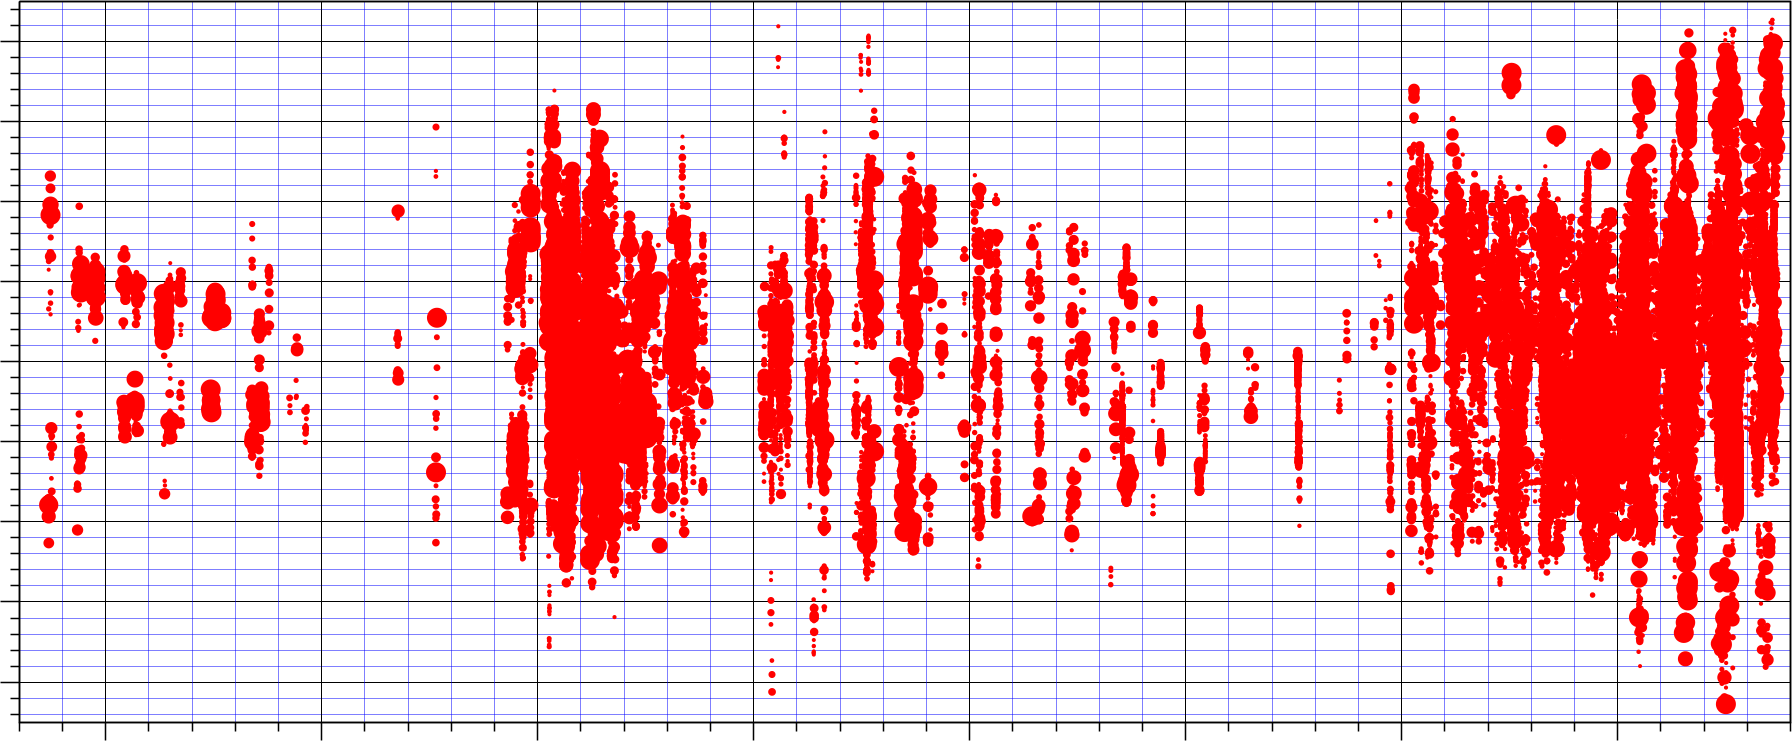
\includegraphics[width=25mm]{hbutterfly.png} \end{tabular}};
%\node[largetextarea, above right=-8mm and 5mm of dbase] (cbutterfly) {\setlength\tabcolsep{0pt} \begin{tabular}{m{23mm}m{25mm}} Dim region butterfly & 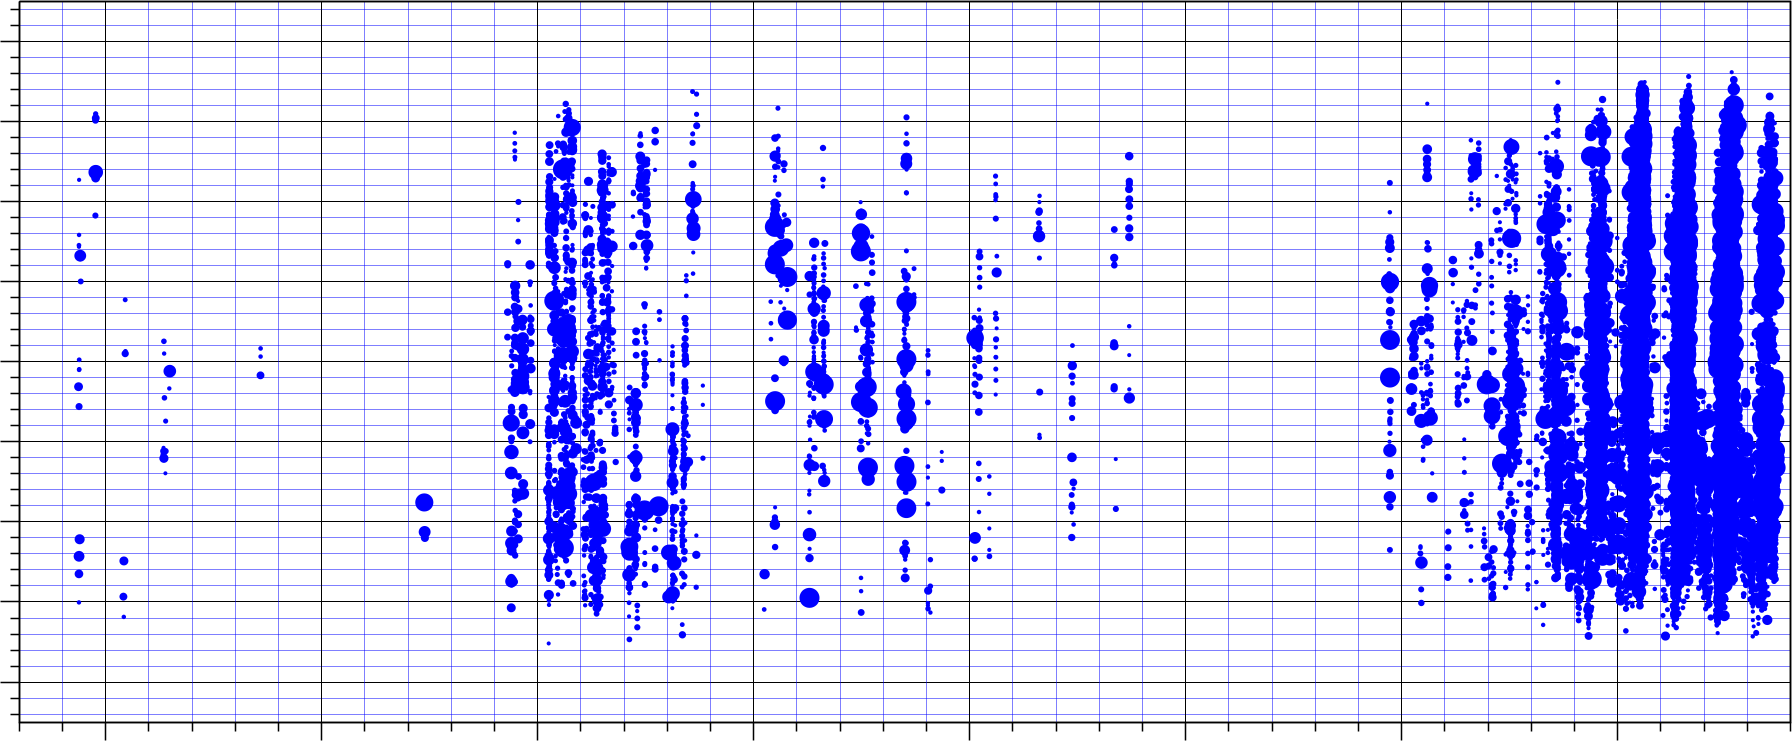
\includegraphics[width=25mm]{cbutterfly.png} \end{tabular}};
%\node[textarea2, right=10mm of hbutterfly] (compu) {Comparison with solar simulations};
%\node[dummy, left=4mm of calib.north] (calib_n1) {};
%\node[dummy, right=4mm of calib.north] (calib_n2) {};
%\node[dummy, left=4mm of calib.south] (calib_s1) {};
%\node[dummy, right=4mm of calib.south] (calib_s2) {};
%\node[dummy, left=4mm of dbase.south] (dbase_s1) {};
%\node[dummy, right=4mm of dbase.south] (dbase_s2) {};
%\node[dummy, left=4mm of estimate.north] (estimate_n1) {};
%\node[dummy, right=4mm of estimate.north] (estimate_n2) {};
%\draw[myarrow] (maps.east) -- (calib.west);
%\draw[myarrow] (calib_s1) -- (estimate_n1);
%\draw[myarrow] (estimate_n2) -- (calib_s2);
%\draw[myarrow] (calib_n1) -- (dbase_s1);
%\draw[myarrow] (dbase_s2) -- (calib_n2);
%\node[dummy, above=4mm of dbase.east] (dbase_e1) {};
%\node[dummy, below=4mm of dbase.east] (dbase_e2) {};
%\draw[myarrow] (dbase_e1) -- (cbutterfly.west);
%\draw[myarrow] (dbase_e2) -- (hbutterfly.west);
%\draw[myarrow] (calib.east) -- (qbutterfly.west);
%\node[dummy, above=6mm of estimate.east] (estimate_e1) {};
%\node[dummy, above=2mm of estimate.east] (estimate_e2) {};
%\node[dummy, below=2mm of estimate.east] (estimate_e3) {};
%\node[dummy, below=6mm of estimate.east] (estimate_e4) {};
%\node[dummy, above=2mm of ibutterfly.west] (ibutterfly_w1) {};
%\node[dummy, below=2mm of ibutterfly.west] (ibutterfly_w2) {};
%\node[dummy, above=2mm of lmodel.west] (lmodel_w1) {};
%\node[dummy, below=2mm of lmodel.west] (lmodel_w2) {};
%\draw[myarrow] (estimate_e1) -- (ibutterfly_w1);
%\draw[myarrow] (ibutterfly_w2) -- (estimate_e2);
%\draw[myarrow] (estimate_e3) -- (lmodel_w1);
%\draw[myarrow] (lmodel_w2) -- (estimate_e4);
%\node[dummy, above=4mm of compu.west] (compu_w1) {};
%\node[dummy, above=0mm of compu.west] (compu_w2) {};
%\node[dummy, below=4mm of compu.west] (compu_w3) {};
%\draw[myarrow] (cbutterfly.east) -- (compu_w1);
%\draw[myarrow] (hbutterfly.east) -- (compu_w2);
%\draw[myarrow] (qbutterfly.east) -- (compu_w3);
%\end{tikzpicture}} \caption{Roadmap for extracting valuable information from the solar maps.} \label{roadmap} \end{figure*}
%

\FloatBarrier

\section{List of symbols} \label{sect:sym}

\skk{At least I need this list in order to keep track of reserved letters. I tried using 'longtable' to automatically 
wrap the table along many pages, but it complains about two column mode. I also tried 'supertabular' but it didn't work 
either. Maybe it is best to manually split the table as I did in my mastersthesis. It is anyway good to assign the 
symbols into groups by relevance.}
\setlength{\extrarowheight}{3pt}
\def\tabularxcolumn#1{m{#1}}
\newcommand{\symtable}[2]{\begin{table*} \caption{#1} \begin{tabularx}{\textwidth}{lX} #2 \end{tabularx} \end{table*}}
\symtable{Disk fitting and signal levels}{
$S$         & A particular \emph{solar map}, also terms \emph{map} and \emph{scan} are used. $S$ is a set of samples. In order to reduce the amount of subscripts and superscripts in various symbols, we often omit the $S$ and assume that it is known from context. \\
$s_i$       & Radio sample in map $S$. It is a bundle of numerical values just as coordinates and intensities. \\
$N_S$       & Number of samples in map $S$. \\
$I_S$       & Index set of $S$: $I_S = \left\{ 1, 2, ..., N_S \right\}$. \\
$i$         & Index used for solar map samples so that $s_i \in S \; \Leftrightarrow \; i \in I_S$. Any numerical value accosiated with $s_i$ is referred with index $i$. \\
$t_i$       & Time when the sample$s_i$ is recorded. Typical unit is unix time in seconds. Recording the map $S$ typically takes a few minutes. \\
$x_i$       & Uncalibrated relative right ascension of the radio sample, with respect to the expected center of the visible solar disk. \\
$y_i$       & Uncalibrated relative declination of the radio sample, with respect to the expected center of the visible solar disk. Cosine corrected. \\
$u_i$       & Uncalibrated, raw intensity of a particular radio sample $s_i$, typically in the range $-4000 .. 32000$. \\
$\RA(s_i)$  & Absolute right ascension of a particular sample, as seen from MRO at time $t_i$. \\
$\Dec(s_i)$ & Absolute declination of a particular sample, as seen from MRO at time $t_i$. \\
$t$         & Time. \\
$\RA_{\astrosun}(t)$  & Absolute right ascension of the center of the solar disk as seen from MRO at time $t$. \\
$\Dec_{\astrosun}(t)$ & Absolute declination of the center of the solar disk as seen from MRO at time $t$. \\
$c$         & Calibration round; calibration involves normalization and centering. We start with $c=0$. \\
$v_i^{(c)}$ & Normalized sample intensity after round $c$. We aim to have zero intensity at the background and unity at the disk. \\
$x^{(c)}$   & \multirow{2}{140mm}{Center of the calibrated map after round $c$.} \\
$y^{(c)}$ \\
$x_i^{(c)}$ & \multirow{2}{140mm}{Calibrated right ascension and declination of sample $s_i$ after calibration round $c$.} \\
$y_i^{(c)}$ \\
$r^{(c)}$   & Radius of the calibrated map after round $c$.}

\symtable{Initial normalization}{
$j$         & Index used for solar map samples when they are sorted by their raw intensity. \\
$u$         & Real value used for uncalibrated intesities. \\
$f_S$       & Bijective mapping $f_S:\; I_S \mapsto I_S$ used for sorting the samples by their raw intensities. \\
$w^{-1}(j)$ & Index v.s. raw intensity in the S-curve method: $w^{-1}(j) = u_{f_S(j)}$ and $j \le j^{\prime} \; \Leftrightarrow \; w^{-1}(j) \le w^{-1}(j^{\prime})$. \\
$w(u)$      & Inverse of $w^{-1}(j)$, raw intensity v.s. sample index. \\
$k$         & Integer used for iterations of the S-curve method, starting with $k=1$. \\
$P_k(u)$    & Polynomial used to approximate $w(u)$ during iteration round $k$. \\
$\s{n}{sc}$ & Degree of $P_k$ approximation for $w(u)$. Typically, $\s{n}{nc} = 3$. Must be odd and at least $3$. \\
$a_n^{(k)}$ & Coefficient of $P_k$. \\
$\bm{a}_k$  & All coefficients of $P_k$ as a vector of $\s{n}{sc}+1$ elements. \\
$T_k(\bm{a}_k)$           & Target function when optimizing the quality of fit for $w(u)$. \\
$\s{j}{min}^{(k)}$        & \multirow{2}{140mm}{Domain of indices used on round $k$.} \\
$\s{j}{max}^{(k)}$ \\
$\s{u}{root}^{(k)}$       & Point of zero curvature, for which $P^{\prime\prime}_k(\s{u}{root}) = 0$. \\
$\s{j}{pivot}^{(k)}$      & Pivot index obtained as $\s{j}{pivot}^{(k)} := P_k(\s{u}{root})$. \\
$\s{u}{background}^{(k)}$ & Background level obtained from S-curve method iteration $k$. \\
$\s{u}{disk}^{(k)}$       & Solar disk level obtained from S-curve method iteration $k$. \\
$\s{u}{background}$       & \multirow{2}{140mm}{Final intensity levels when we have terminated the S-curve iteration.} \\
$\s{u}{disk}$}

\symtable{Initial centering and radius}{
$b_i^{(c)}$              & Sample weight during calibration round $c$. \\
$\mathcal{B}(\bm{0},R)$  & Disk of radius $R$ centered at origin. \\
$t_S$              & Average observational time during recording $S$. \\
$r_{\astrosun}(t)$ & Apparent radius of the Sun at time $t$. \\
$R_{\astrosun}$    & Physical, three-dimensional radius of the Sun. Depends on wavelength of observation and on exact definition. \\
$d(t)$             & Physical distance between the center (core) of the Sun and MRO during observation at time $t$.}

\symtable{Inner disk outliers}{
$q$                       & Iteration round number, starting with $q=0$, when neglecting inner disk outliers. \\
$\Lambda$                 & Rectangular lattice, a set of lattice points superimposed over the visible solar disk. \\
$I_{\Lambda}$             & Index set for lattice points. \\
$h$                       & Index for rectangular lattice points. \\
$\lambda_h$               & Individual lattice point with $h \in I_{\Lambda}$ and $\Lambda = \left\{ \lambda_h :\; h \in I_{\Lambda}\right)$. \\
$\s{n}{grid}$             & Grid size for the lattice.\\
$\s{x}{min}$              & \multirow{4}{140mm}{Box spanning a two-dimensional range of right ascension and declination. Each sample in scan $S$ fits within this box such that $\s{x}{min} = \min{x_i}$, $\s{x}{max} = \max{x_i}$, $\s{y}{min} = \min{y_i}$, and $\s{y}{max} = \max{y_i}$. This frames the lattice $\Lambda$ and covers the solar disk.} \\
$\s{x}{max}$ \\
$\s{y}{min}$ \\
$\s{y}{max}$ \\
$h_x$                     & \multirow{2}{140mm}{Two-dimensional index for lattice points: $0 \le h_x,h_y < \s{n}{grid}$ with $h_x,h_y \in \mathds{N}$.} \\
$h_y$ \\
$x_h$                     & \multirow{2}{140mm}{Right ascension and declination of the lattice point $h$ with $\s{x}{min} \le x_h \le \s{x}{max}$ and $\s{y}{min} \le y_h \le \s{y}{max}$.} \\
$y_h$ \\
$i_{\Lambda}(h)$          & Maps the lattice index $h \in I_{\Lambda}$ into the map index $i \in I_S$ of the nearest uncalibrated sample. \\
$d_h^{(c)}$               & Distance between lattice point $\lambda_h$ and nearest sample $s_i$ at calibration round $c$. \\
$u_h^{(c)}$               & Lattice point intensity during calibration round $c$. \\
$I_c$                     & Subset of the lattice which contains the inner disk. \\
$I_c^{(q)}$               & Subset of $I_c$ so that bright and dim features are omitted, starting from $q=0$ with $I_c^{(0)} := I_c$. \\
$\s{u}{QSL}^{(c,q)}$      & Quiet Sun Level defined after $q$ outlier iterations during calibration round $c$. \\
$\s{\sigma}{QSL}^{(c,q)}$ & Standard deviation, outliers neglected, after $q$ iterations during calibration round $c$. \\
$\s{q}{max}$              & Number of iterative outlier neglection rounds. \\
$\s{u}{QSL}^{(c)}$        & QSL after outliers neglected from inner disk: $\s{u}{QSL}^{(c)} = \s{u}{QSL}^{(c,\s{q}{max})}$. \\
$\s{\sigma}{QSL}^{(c)}$   & QSL standard deviation after outliers neglected from inner disk: $\s{\sigma}{QSL}^{(c)} = \s{\sigma}{QSL}^{(c,\s{q}{max})}$.}

\symtable{Bright and dim features}{
$I_c^{(\mathrm{dim})}$    & Lattice subset that consists of dim features. \\
$I_c^{(\mathrm{QSL})}$    & Lattice subset that contains no significant features. It is the based on the previous centering round as $I_c^{(\mathrm{QSL})} = I_{c-1}^{(\s{q}{max}+1)}$. \\
$I_c^{(\mathrm{bright})}$ & Lattice subset that consists of bright features. \\
$\mathcal{F}_c$           & Set of features obtained from calibration round $c$. \\
$F$                       & Particular feature $F \in \mathcal{F}_c$. \\
$A(F)$                    & Area of a feature $F$. \\
$r(F)$                    & Radius of a feature $F$. \\
$z(F)$                    & Two-dimensional location of a feature $F$.}

\symtable{Limb outliers}{
$r_i^{(c)}$               & Relative radial distance of sample $s_i$ from the visual center of the solar disk, based on previous calibration round $c-1$. \\
$L^{(c)}_1$               & Samples in $S$ which are not too close to any bright or dim feature. \\
$L^{(c)}_2$               & Samples which are located at the limb by $\pm 0.04$radii. \\
$L^{(c)}_3$               & Samples with intensities between $0.05$ and $0.95$ QSL. \\
$L^{(c)}$                 & Boundary subset used for centering: $L^{(c)} := L^{(c)}_1 \cap L^{(c)}_2 \cap L^{(c)}_3$. \\
$r_i^{\prime(c)}$         & Estimated relative radial distance for sample $s_i \in L^{(c)}$, based on known limb profile, on round $c$. \\
$p$                       & Grand iteration round for optimizing limb profile. This involves processing all the maps of one solar cycle. \\
$l_{p,S}(r)$              & Limb profile for map $S$: estimated intensity at radius $r$ from the center of the solar disk. The profile is a result of chromospheric limb brightning and telescope beam spreading due to diffraction and scattering at Earth's atmosphere. \\
$l_{0,S}(r)$              & Simple limb profile for bootstrapping the grand iteration at $p=0$. It is identical for all maps. \\
$a_{\astrosun}(t)$        & Altitude of the center (core) of the Sun, angle above horizon, as seen from MRO at time $t$. \\
$a_S$                     & Altitude when observing map $S$: $a_S := a_{\astrosun}(t_S)$. \\
$m$                       & Round for iterating the limb profile on a particular $p$, using maps of one solar cycle. \\
$\bm{x}_m^{(p)}$          & Parameter set for the limb model, optimizing at round $m$ and grand iteration $p$. \\
$\kappa$                  & Constant for deciding the level of detail we want for the limb model. \\
$\rho(r)$                 & Transformation for emphasing details at $r=1$: $\rho(r) = \kappa \arctan \left( r - 1 \right)$. \\
$B(\bm{x},\rho,a)$        & Two-dimensional polynomial of $\rho$ and $a$ with desired degree and coefficients included in $\bm{x}$. \\
$\delta r_i^{(c)}$        & Radial error for sample $s_i$: $\delta r_i^{(c)} := r_i^{(c)} - r_i^{\prime(c)}$. \\
$g$                       & Round for negleting limb outliers. We start from $g=4$. \\
$\s{g}{out}$              & Maximum outlier neglection round when there are $\s{g}{out} - 4$ such rounds. \\
$\Delta \left( L^{(c)}_g \right)$ & Standard deviation of radial errors on rounds $g$ and $c$.}

\symtable{Subsequent centering}{
$T_g$ & Quality of circle fitting.}



\FloatBarrier


\begin{acknowledgements}
\end{acknowledgements}


% WARNING
%-------------------------------------------------------------------
% Please note that we have included the references to the file aa.dem in
% order to compile it, but we ask you to:
%
% - use BibTeX with the regular commands:
%   \bibliographystyle{aa} % style aa.bst
%   \bibliography{Yourfile} % your references Yourfile.bib
%
% - join the .bib files when you upload your source files
%-------------------------------------------------------------------

\bibliographystyle{aa}
\bibliography{main_P1}

\end{document}

